\chapter{Réalisation et présentation de la plateforme}

\section*{Introduction}

Ce chapitre décrit le passage de la conception à une plateforme utilisable par un recruteur. L'enjeu n'est pas de reprendre l'architecture logique ni les calculs présentés précédemment, mais de montrer comment ils sont rendus accessibles par une application Web cohérente : saisie des données, exécution d'une évaluation, restitution expliquée et conservation des résultats. Les éléments décrits ci-après proviennent de la version courante du dépôt JobTest ; l'ancienne interface Streamlit est donc considérée comme un prototype et non comme l'interface finale.

\section{Environnement matériel et logiciel}

\subsection{Environnement matériel}

J'ai réalisé le développement, les validations locales et la rédaction de ce mémoire sur mon ordinateur personnel, décrit ci-dessous. Cet environnement local est distinct de la machine virtuelle Azure décrite au chapitre~6 ; aucune mesure de performance matérielle n'est déduite de ces caractéristiques.

Le tableau~\ref{tab:chap5-hardware} en donne les caractéristiques.

\begin{table}[H]
\centering
\small
\caption{Environnement matériel}
\label{tab:chap5-hardware}
\begin{tabularx}{.82\textwidth}{|p{.34\textwidth}|X|}
\hline
\textbf{Composant} & \textbf{Caractéristique}\\ \hline
Ordinateur & HP\\ \hline
Processeur & Intel Core i3, 11\textsuperscript{e} génération\\ \hline
Mémoire vive & 8 Go de RAM\\ \hline
Processeur graphique & Intel UHD Graphics\\ \hline
Stockage total & Environ 1 300 Go\\ \hline
\end{tabularx}
\end{table}

\subsection{Environnement logiciel}

Le développement associe un service Python et une application Web Next.js. L'environnement local s'appuie sur Windows, Python, Node.js et \texttt{npm}. L'API est exécutée avec Uvicorn ; le navigateur sert à vérifier les parcours de l'interface. Git est utilisé pour le suivi des sources. Les versions expressément verrouillées par le projet sont indiquées ; aucune version non vérifiable de système, d'éditeur ou de navigateur n'est inférée.

Le tableau~\ref{tab:chap5-environment} récapitule ces outils et le rôle tenu par chacun.

\begin{table}[H]
\centering
\small
\caption{Environnement de réalisation}
\label{tab:chap5-environment}
\begin{tabularx}{\textwidth}{|l|l|X|}
\hline
\textbf{Élément} & \textbf{Outil ou technologie} & \textbf{Rôle dans le projet}\\
\hline
Système local & Windows & Développement et exécution locale des services.\\
\hline
Backend & Python, FastAPI et Uvicorn & Exposition de l'API, services métier et exécution ASGI.\\
\hline
Frontend & Next.js 14.2.35, React 18, TypeScript & Pages App Router, composants et interactions du recruteur.\\
\hline
Styles et animation & Tailwind CSS, Framer Motion & Système visuel, états de l'interface et transitions.\\
\hline
Données locales & SQLite et SQLAlchemy & Persistance locale des comptes, offres, candidats, CV et évaluations.\\
\hline
Outils IA & scikit-learn, Sentence-Transformers, spaCy, Ollama & Moteur de rapprochement et analyse qualitative optionnelle.\\
\hline
Documents & ReportLab & Construction du rapport PDF d'évaluation.\\
\hline
Conteneurs & Docker Compose, Caddy, PostgreSQL & Environnement de déploiement ; détaillé au chapitre 6.\\
\hline
\end{tabularx}
\end{table}

\section{Choix des technologies}

Les choix présentés dans cette section sont justifiés par les responsabilités effectivement portées par chaque partie de JobTest.

\subsection{Technologies frontend}

Le répertoire \texttt{web/} contient le frontend final. Next.js organise les écrans dans \texttt{app/}, selon l'App Router, et React porte les composants réutilisables. TypeScript définit les contrats manipulés par le client API et évite que les données de réponse soient traitées comme des objets non structurés. Les routes principales correspondent notamment à la connexion, à la vue d'ensemble, aux offres, aux candidats, à l'analyse, à l'historique, au classement et au centre de qualité.

Tailwind CSS est employé pour composer les styles de l'interface et les variantes des composants communs, tels que boutons, cartes, tableaux, badges, champs et états vides. Framer Motion est utilisé pour les transitions de pages, l'apparition du résultat et les animations de score. Le projet référence également Three.js, \texttt{@react-three/fiber} et \texttt{@react-three/drei} ; leur emploi est concret dans les éléments graphiques \texttt{AmbientBackground}, \texttt{ScoreTorus} et \texttt{NeuralField}. Ces éléments complètent la lecture visuelle du score sans porter la décision elle-même.

\subsection{Technologies backend}

FastAPI regroupe l'API sous le préfixe \texttt{/api/v1}. L'application installe les routeurs d'authentification et le routeur \texttt{/api/v1/ui}, destiné aux besoins du frontend actuel. Les modèles Pydantic définissent et valident les corps des requêtes, par exemple une offre, une évaluation ou une demande de rapport. La séparation rend explicites les entrées HTTP avant l'appel aux services de rapprochement.

SQLAlchemy représente les entités \emph{User}, \emph{Candidate}, \emph{CV}, \emph{JobOffer}, \emph{MatchResult} et \emph{Skill}. Les relations lient le candidat à ses CV et ses résultats, et le recruteur à ses propres candidats et offres. Les contrôles de propriété appliqués par l'API empêchent qu'un identifiant d'offre ou de candidat appartenant à un autre recruteur soit utilisé dans une évaluation.

Le parsing des CV repose sur \texttt{pdfplumber} avec repli \texttt{PyPDF2} pour les PDF, et sur \texttt{python-docx} avec repli XML pour les documents Word. ReportLab génère le PDF à partir des données déjà calculées : en-tête, identité affichée, score, radar, compétences, écarts, recommandations et aide à la décision. La génération reste ainsi découplée de l'affichage Next.js.

L'authentification s'appuie sur des jetons JWT transmis dans l'en-tête \texttt{Authorization: Bearer}. Le client conserve le jeton dans le stockage local du navigateur et l'ajoute aux appels protégés. Les mots de passe ne sont pas retournés par les endpoints ; seul le hachage est conservé dans le modèle utilisateur.

\subsection{Technologies d'intelligence artificielle}

Le premier niveau d'analyse mobilise les composants décrits au chapitre~\ref{chap:moteur-intelligent} : TF--IDF de scikit-learn, similarité sémantique avec Sentence-Transformers, extraction et rapprochement de compétences, puis fusion hybride. spaCy intervient lorsqu'un modèle linguistique est disponible, avec une stratégie de repli dans le prétraitement. Le chargement des services est différé jusqu'à la première requête nécessitant le moteur, ce qui permet à l'API de démarrer sans calculer immédiatement les modèles.

La seconde couche qualitative est appelée après l'affichage du résultat principal. Le runtime local Ollama est configuré avec \texttt{qwen2.5:1.5b}. Son indisponibilité n'empêche pas l'évaluation statistique : la réponse expose alors un état contrôlé tel que \emph{unavailable}, \emph{disabled} ou \emph{error}. Cette distinction est importante pour l'utilisateur : l'analyse approfondie enrichit la lecture, mais ne modifie ni le score ni le verdict du premier niveau.

\subsection{Technologies de données et d'infrastructure}

SQLite constitue le choix par défaut en développement local grâce à une base fichier et à l'intégration SQLAlchemy. Pour l'environnement conteneurisé, le fichier \texttt{docker-compose.yml} définit PostgreSQL 16 comme service de données. Docker Compose réunit également l'API, l'application Web, Ollama et le proxy inverse. Dans la version déployée, ce proxy est Caddy, point d'entrée HTTPS ; il relaie les chemins \texttt{/api/v1/} vers FastAPI et les autres chemins vers Next.js. La procédure complète de sécurisation, de conteneurisation et de déploiement sur machine virtuelle Azure est réservée au chapitre 6.

Le tableau~\ref{tab:chap5-technology-summary} synthétise ces choix et l'usage qui en est réellement fait.

\begin{table}[H]
\centering
\small
\caption{Choix techniques}
\label{tab:chap5-technology-summary}
\begin{tabularx}{\textwidth}{|l|l|X|}
\hline
\textbf{Domaine} & \textbf{Technologie} & \textbf{Utilisation réelle dans JobTest}\\
\hline
Interface & Next.js, React, TypeScript & Écrans App Router, composants et client HTTP.\\
\hline
Présentation & Tailwind CSS, Framer Motion, Three.js & Styles, transitions et représentations visuelles du score.\\
\hline
API & FastAPI, Pydantic & Endpoints, validation et sérialisation JSON.\\
\hline
Persistance & SQLAlchemy, SQLite / PostgreSQL & Entités métier et stockage selon l'environnement.\\
\hline
Rapprochement & scikit-learn, Sentence-Transformers, spaCy & Signaux lexical, sémantique et compétences.\\
\hline
Analyse qualitative & Ollama, Qwen & Analyse approfondie non bloquante.\\
\hline
Export & ReportLab & Rapport PDF téléchargeable.\\
\hline
\end{tabularx}
\end{table}

\section{Organisation du code source}

L'organisation privilégie la séparation entre interface, API, règles de rapprochement et accès aux données. L'arborescence simplifiée suivante ne montre que les dossiers participant directement au fonctionnement de la version étudiée.

\begin{verbatim}
web/                 pages Next.js, composants, client API et styles
src/api/             application FastAPI et routeurs auth / UI
src/matching/        service d'évaluation et persistance du résultat
src/models/          TF-IDF, embeddings, compétences et chargement
src/fusion/          score hybride
src/decisioning/     règles de verdict
src/explainability/  explication et recommandations structurées
src/ai/              prompts et analyse qualitative Ollama
src/parsing/         extraction PDF/DOCX et nettoyage
src/reporting/       génération ReportLab
src/models_db.py     modèles SQLAlchemy
deploy/Caddyfile     proxy inverse HTTPS
\end{verbatim}

Le frontend ne recopie pas les règles du moteur. Son fichier \texttt{lib/api/client.ts} centralise les appels HTTP et les types associés. Côté API, le routeur de parité UI traduit les requêtes de l'interface vers le même service métier que les endpoints techniques. Cette organisation limite les divergences entre un calcul réalisé depuis un écran et un calcul réalisé par API.

\section{Réalisation du backend}

L'initialisation FastAPI crée les tables lorsqu'elles sont absentes et applique une vérification additive de schéma. Les routeurs couvrent l'inscription, la connexion, la lecture de l'utilisateur courant, les offres, les candidats, les résultats, l'évaluation, l'analyse approfondie, la comparaison des modèles, les indicateurs et le rapport PDF. Un middleware ajoute un identifiant de requête, mesure le temps de traitement et applique une limitation de fréquence en mémoire.

Le routeur UI fournit les opérations nécessaires aux pages : lecture et création d'offres, modification de leur statut, consultation et modification des candidats, lecture d'historique, évaluation textuelle ou par fichier, et lecture des indicateurs. Lors d'une évaluation, l'API vérifie l'offre sélectionnée, le contenu minimal du CV et l'appartenance des données au recruteur connecté. Le service \texttt{evaluate\_and\_persist} calcule le résultat, crée ou retrouve le candidat selon les données fournies, conserve le CV et enregistre les sous-scores, le verdict, les seuils actifs et l'explication JSON.

La route de rapport reçoit les objets déjà calculés et renvoie un flux \texttt{application/pdf} avec un en-tête de téléchargement. Ce choix évite de recalculer le matching lors de l'export. De manière analogue, la route d'analyse approfondie reçoit l'identifiant d'un résultat persistant, reconstruit son contexte et renvoie une enveloppe d'état sans faire échouer le parcours lorsque le LLM n'est pas accessible.

\section{Réalisation du frontend}

La zone authentifiée est enveloppée par un layout commun : barre latérale, barre supérieure, transition de page et zone centrale. Au chargement, le layout vérifie la présence du jeton puis appelle \texttt{/auth/me}. En cas d'échec, il redirige vers la connexion. Cette vérification protège l'expérience utilisateur au niveau de l'interface, tandis que l'API vérifie de nouveau le jeton pour chaque ressource protégée.

Les pages utilisent des composants génériques pour maintenir une restitution homogène. \texttt{Table} porte les listes, \texttt{Modal} les opérations de modification ou de confirmation, \texttt{Field} les saisies, et \texttt{DataStates} les états de chargement ou d'absence de données. Les pages d'offres et de candidats affichent leurs données sous forme de tableau et appellent le client centralisé pour actualiser leur état après une modification. Les erreurs réseau ou fonctionnelles sont converties en notifications visibles ; le bouton de l'évaluation affiche également un état de travail pendant le calcul.

La page d'analyse regroupe la sélection d'une offre ouverte, le choix de méthode, l'identité facultative du candidat et deux modes d'entrée du CV : collage de texte ou téléversement PDF/DOCX. Après la réponse JSON, elle révèle le score, le verdict, les composantes, le radar de compétences, les forces, lacunes et recommandations. L'export PDF transmet les données du résultat vers le backend. Le composant \texttt{DeepAnalysis} déclenche séparément la couche qualitative et présente son état sans masquer la restitution du premier niveau.

\section{Intégration frontend--backend}

Le parcours d'une évaluation relie deux responsabilités complémentaires. Le navigateur assure la collecte et la restitution ; le serveur possède les règles métier et les données persistantes.

\begin{enumerate}
  \item Le recruteur choisit une offre et saisit ou téléverse le CV dans l'écran \emph{Candidate Analysis}.
  \item Le frontend contrôle les informations requises et construit une requête vers \texttt{/api/v1/ui/evaluate} ou \texttt{/api/v1/ui/evaluate/file}.
  \item Le client API ajoute le jeton bearer, puis FastAPI valide le schéma Pydantic, l'utilisateur et la propriété de l'offre.
  \item Le service métier extrait éventuellement le document, exécute le moteur de niveau 1 et produit explication, recommandations et décision.
  \item SQLAlchemy conserve le candidat, le CV et le résultat lorsque le parcours est persistant.
  \item La réponse JSON est affichée par les composants de score ; l'analyse approfondie est demandée indépendamment après cette réponse.
  \item Sur demande, le frontend envoie les éléments nécessaires à \texttt{/api/v1/report/pdf} et télécharge le document retourné.
\end{enumerate}

En développement, le client pointe vers l'API locale configurée par \texttt{NEXT\_PUBLIC\_API\_BASE}. Dans le déploiement, le même chemin relatif \texttt{/api/v1} est servi derrière le proxy inverse, ce qui évite d'exposer au navigateur les adresses internes des conteneurs. Les réponses d'erreur HTTP sont transformées en messages d'interface ; l'état particulier de la Layer 2 est, lui, affiché comme une disponibilité de service et non comme un échec de l'évaluation principale.

\section{Présentation des interfaces}

J'ai réalisé les captures de cette section sur une instance locale exécutant la version finale du code (modèle \texttt{hybrid-checkpoint-v4} et calibration versionnée livrée). Je les ai produites avec le navigateur Chrome, piloté par un script du dépôt (\texttt{scripts/capture\_screens.py}), dans une fenêtre de 1\,440 $\times$ 900 pixels, sans autre retouche que le masquage des dates. Pour la lisibilité, la barre de navigation latérale, identique sur toutes les pages et visible sur la figure~\ref{fig:chap5-overview}, est recadrée sur les autres écrans de l'application. Le jeu de démonstration est entièrement fictif~: compte recruteur de test, offres rédigées pour l'occasion, candidats dotés d'adresses \texttt{example.com} et dix-huit CV fictifs au format PDF. Aucun CV personnel n'y figure.

\subsection{Connexion et identité visuelle}

La page de connexion comporte les champs courriel et mot de passe, un lien de création de compte et une notification d'erreur en cas d'échec. Les champs sont vides à l'ouverture. La partie visuelle présente l'identité JobTest et le rôle d'aide au recrutement. Après authentification, l'utilisateur est dirigé vers la vue d'ensemble (figure~\ref{fig:chap5-login}).

\begin{figure}[H]
  \centering
  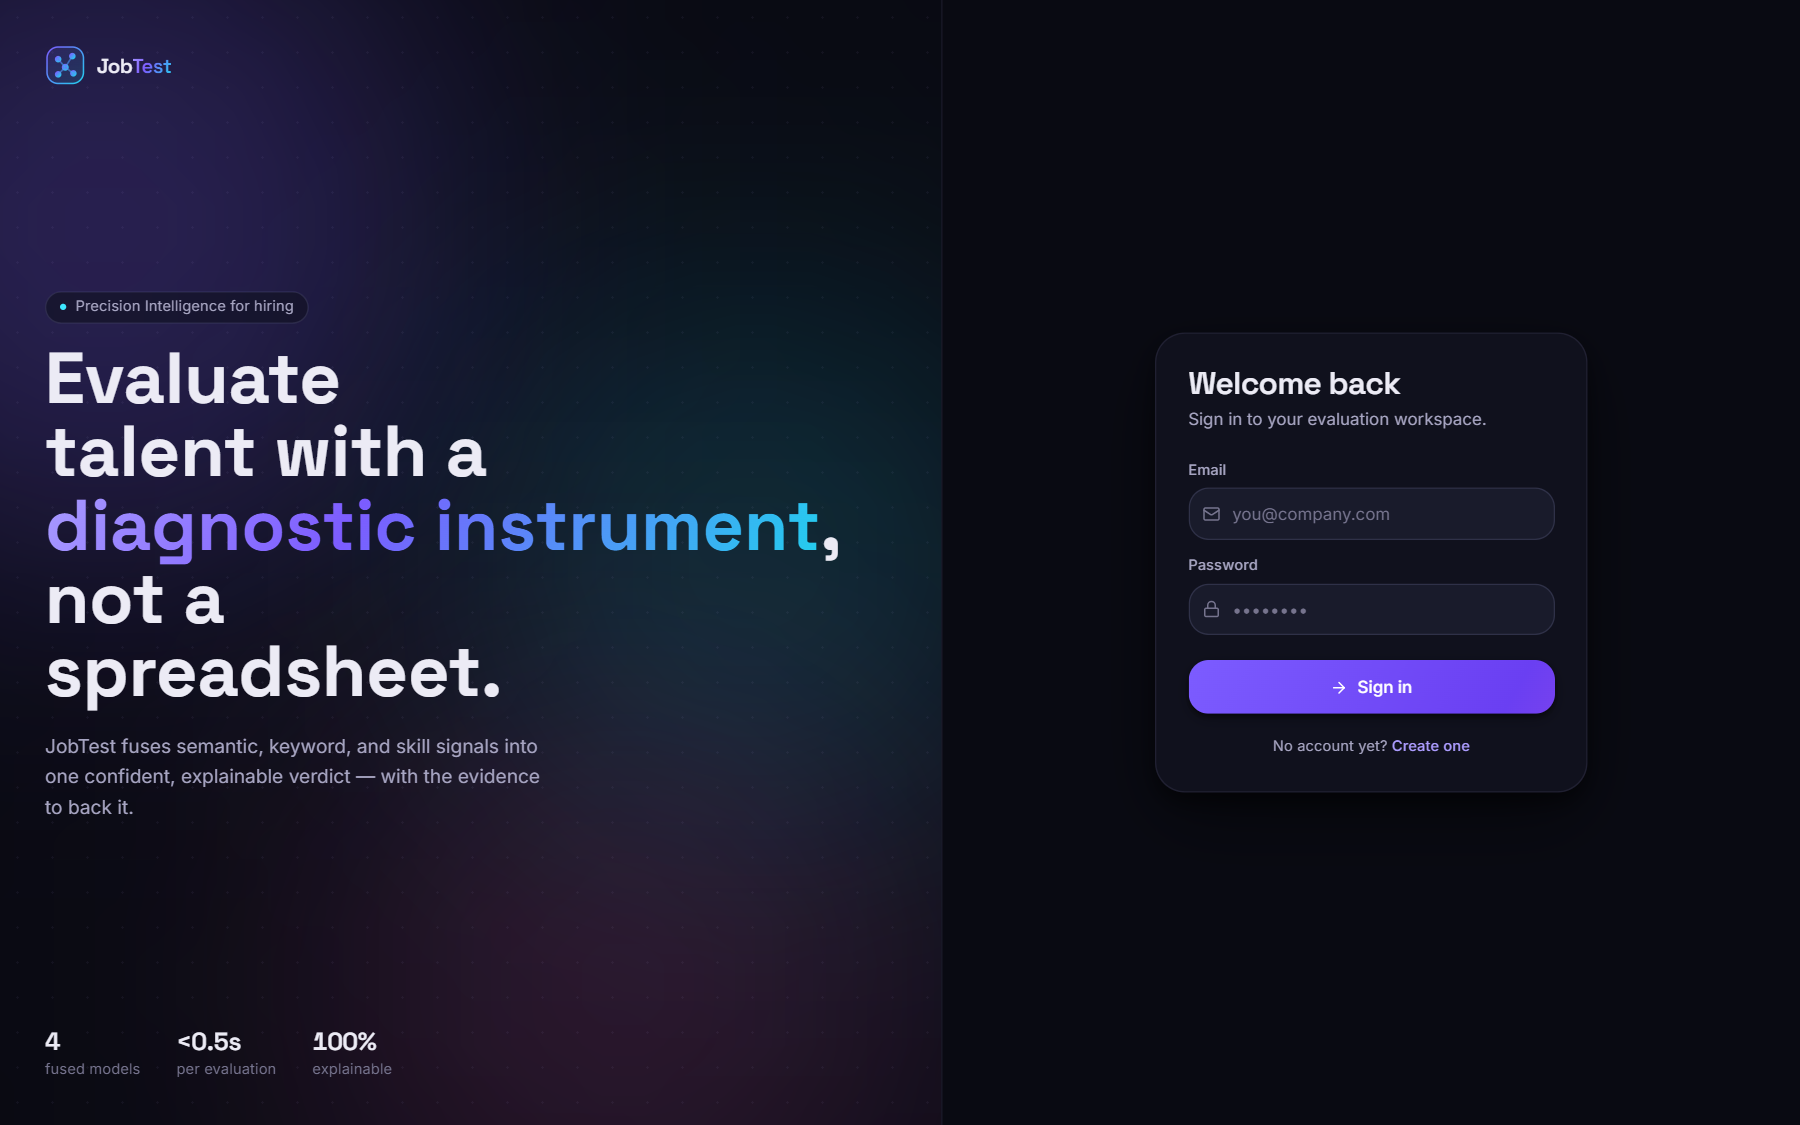
\includegraphics[width=.95\textwidth]{img/interfaces/login.png}
  \caption{Écran de connexion}
  \label{fig:chap5-login}
\end{figure}

L'inscription est proposée sur ce même écran~; elle demande le nom, le courriel, le mot de passe et sa confirmation (figure~\ref{fig:chap5-register}).

\begin{figure}[H]
  \centering
  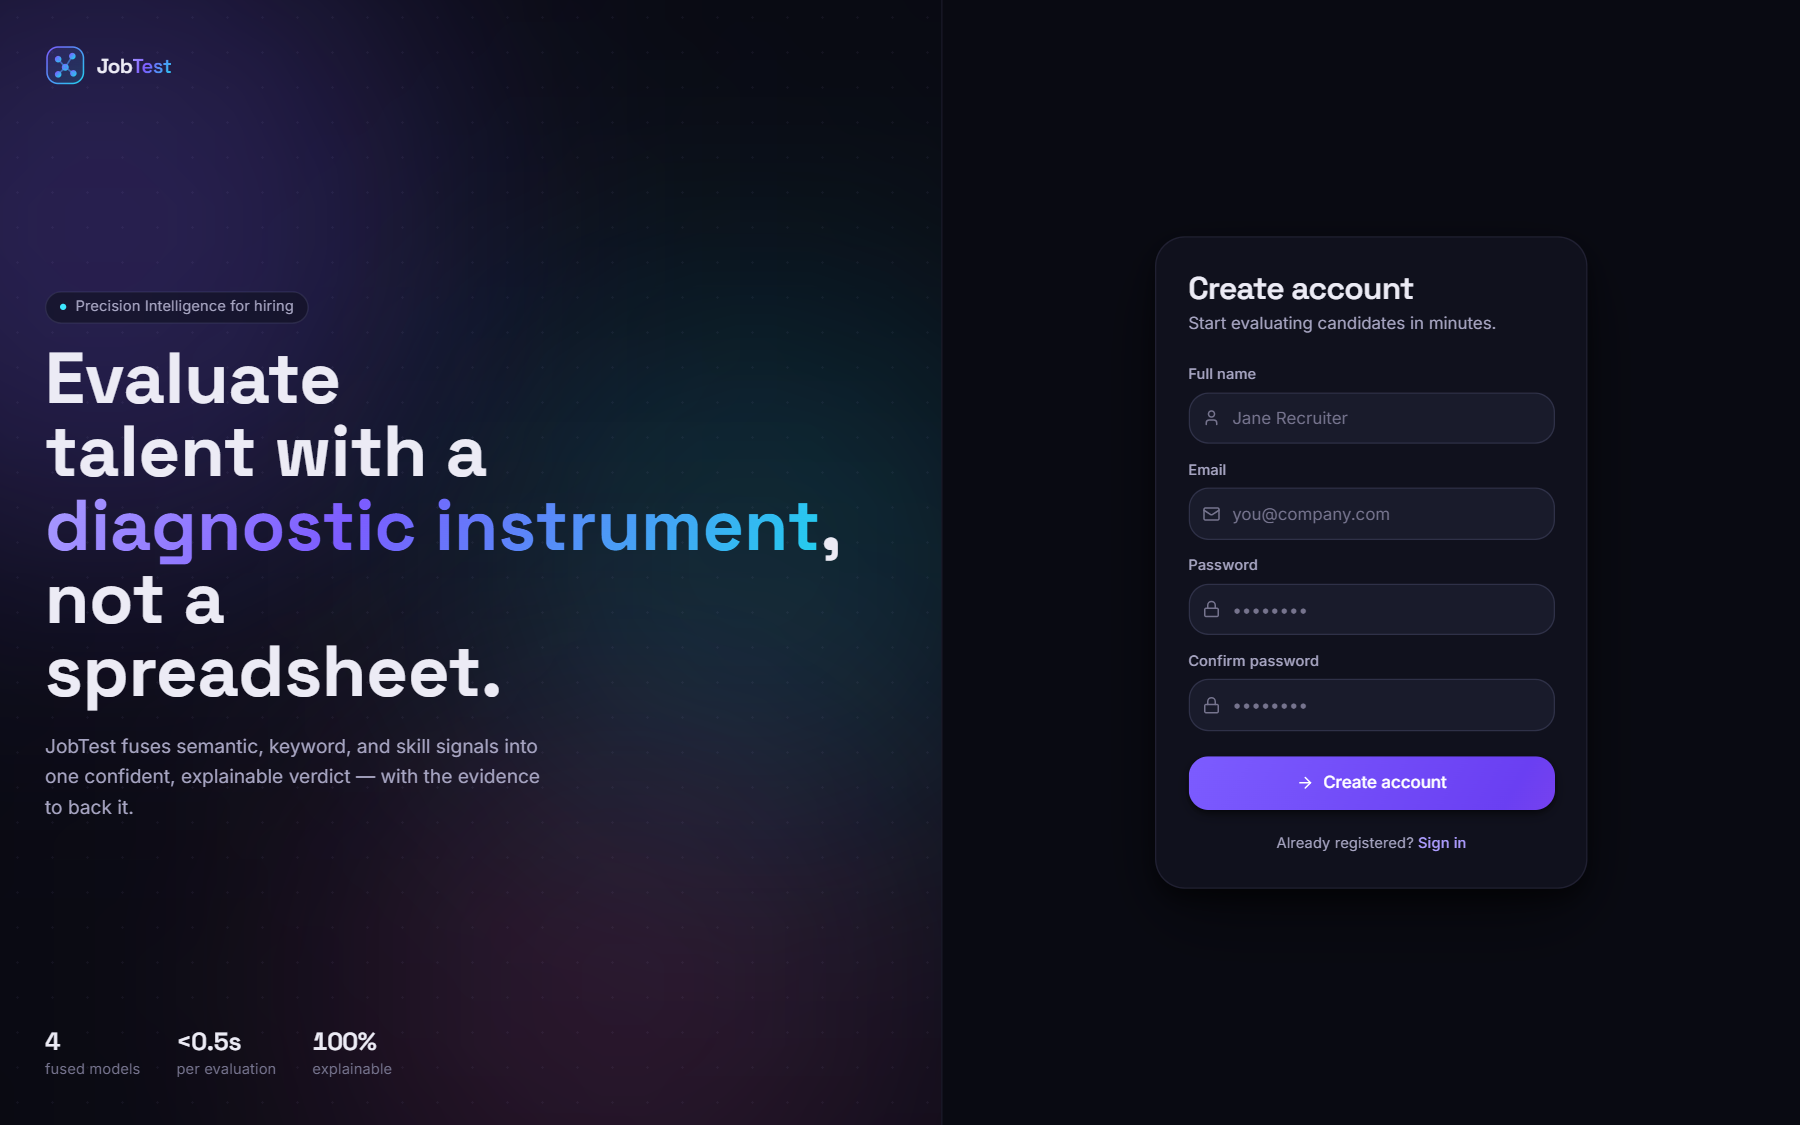
\includegraphics[width=.95\textwidth]{img/interfaces/register.png}
  \caption{Écran d'inscription}
  \label{fig:chap5-register}
\end{figure}

\subsection{Consultation sur mobile}

La mise en page s'adapte aux écrans étroits~: la barre latérale laisse place à une navigation horizontale et les grilles passent sur une colonne, sans modifier les règles métier ni les résultats fournis par l'API. La figure~\ref{fig:chap5-mobile-1} montre la vue d'ensemble et l'historique à la largeur d'un téléphone, obtenus par l'émulation mobile du navigateur (390 pixels de large).

\begin{figure}[H]
  \centering
  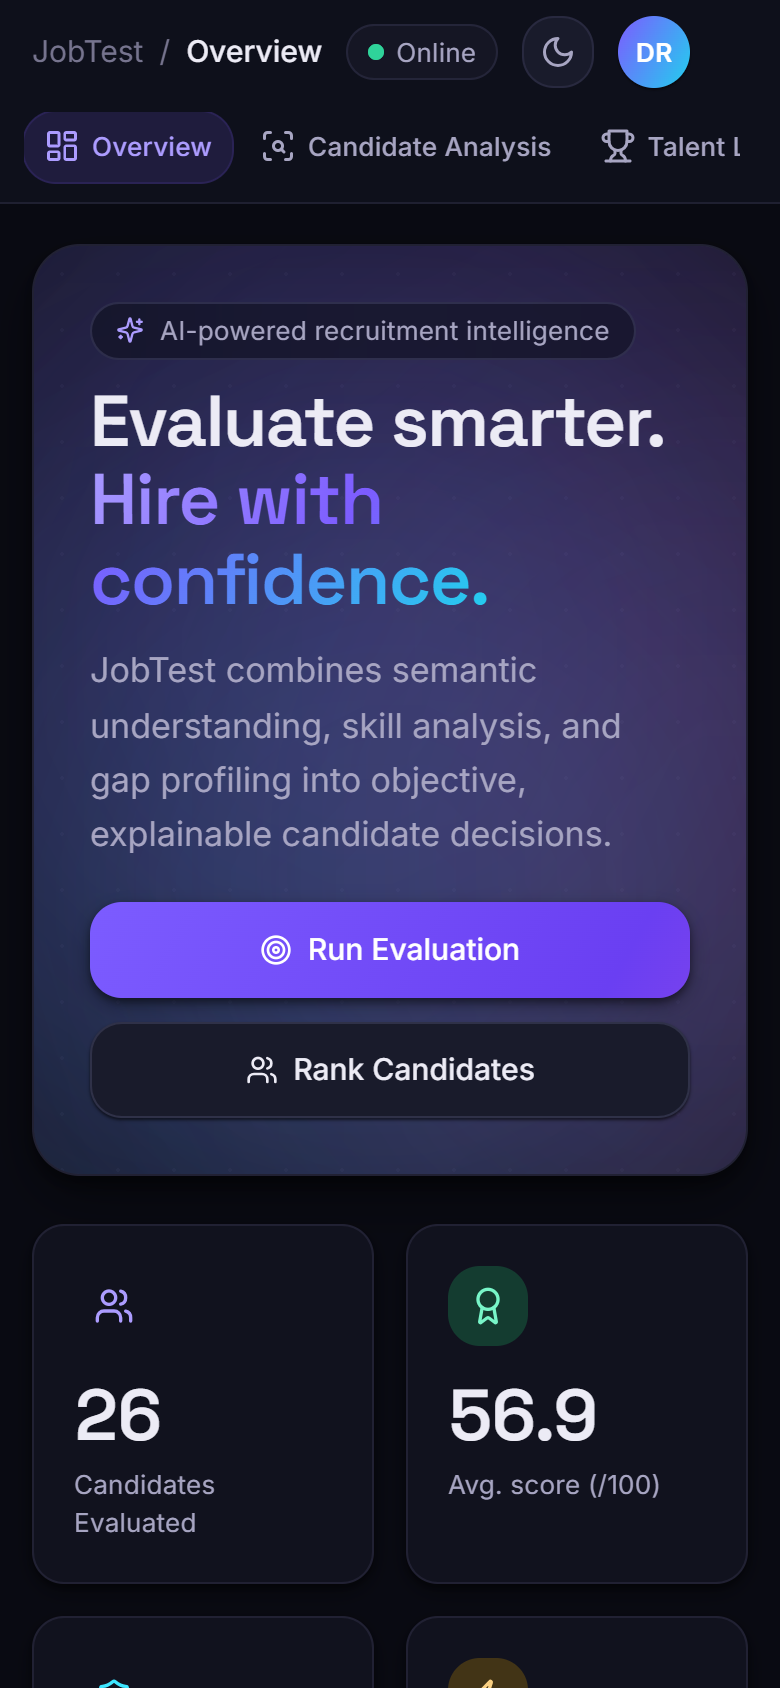
\includegraphics[width=.34\textwidth]{img/interfaces/phone_1.png}\hspace{1.2cm}%
  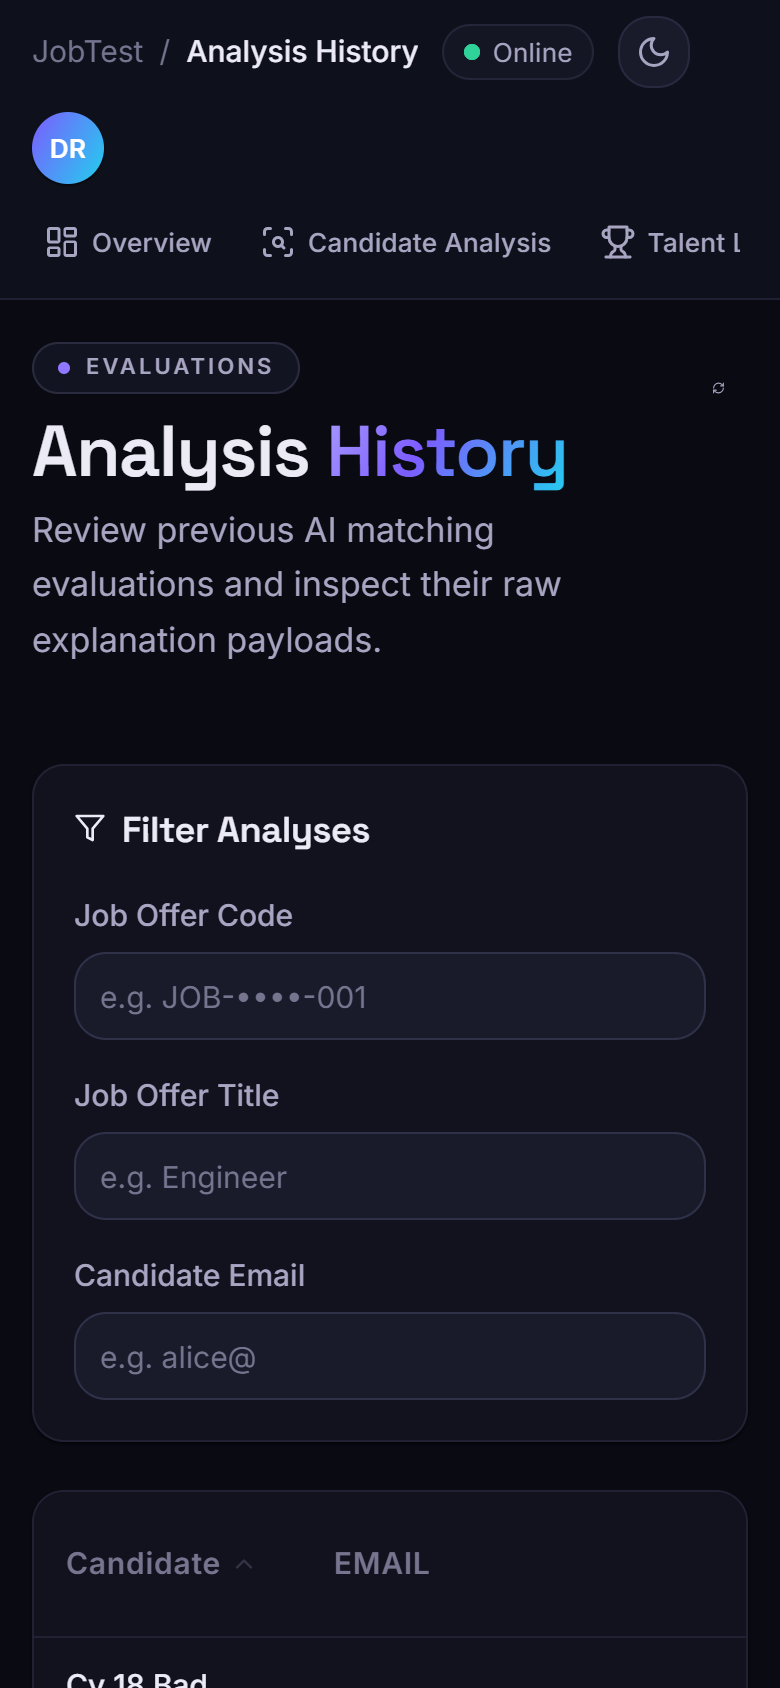
\includegraphics[width=.34\textwidth]{img/interfaces/phone_2.png}
  \caption{Affichage en largeur mobile}
  \label{fig:chap5-mobile-1}
\end{figure}

\subsection{Vue d'ensemble, offres et candidats}

La vue \emph{Overview} synthétise le nombre de candidats, le nombre d'offres, le nombre d'évaluations, le score calibré moyen sur 100 ainsi que la part des verdicts \texttt{HIRE}, puis les résultats récents et la répartition des verdicts. Ces valeurs sont calculées côté API à partir des objets appartenant au recruteur connecté, et seuls les résultats calculés sur l'échelle calibrée entrent dans les moyennes (figure~\ref{fig:chap5-overview}).

\begin{figure}[H]
  \centering
  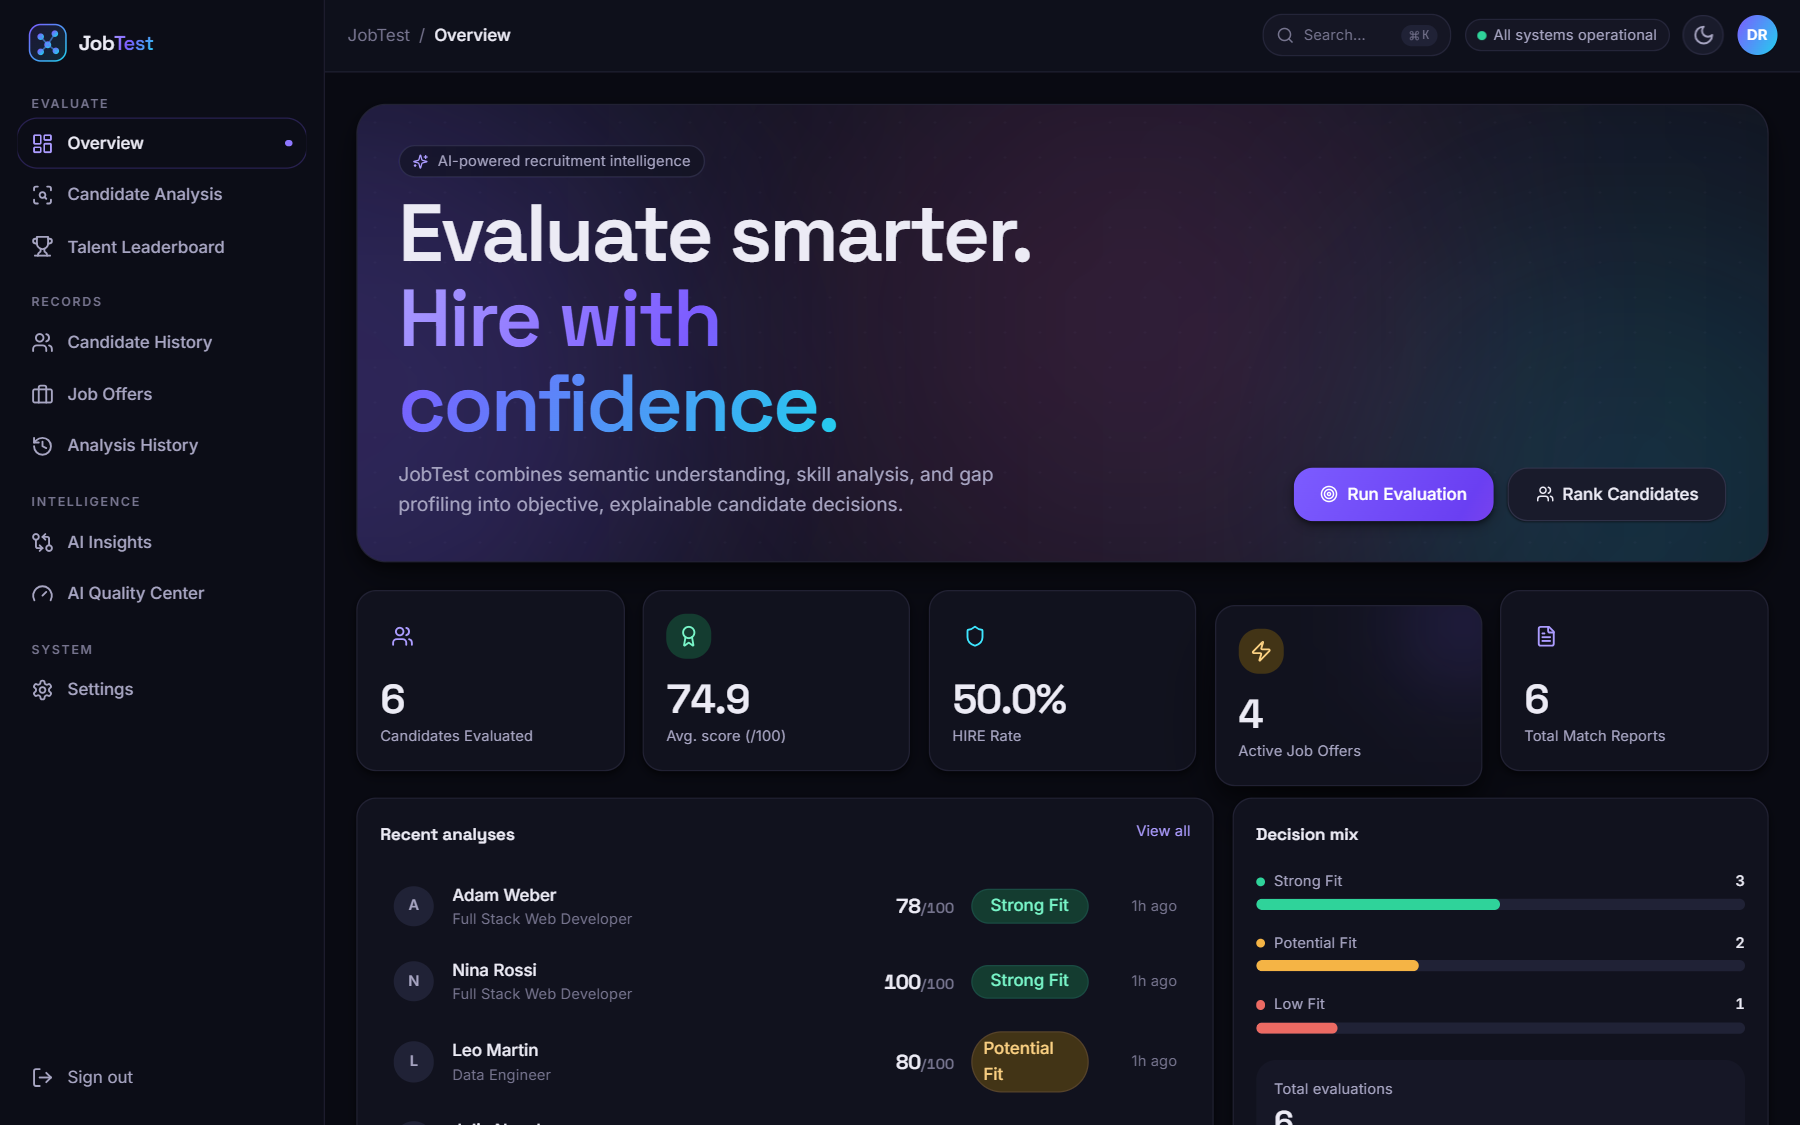
\includegraphics[width=.95\textwidth]{img/interfaces/overview.png}
  \caption{Vue d'ensemble}
  \label{fig:chap5-overview}
\end{figure}

La figure~\ref{fig:chap5-search} illustre la recherche transversale accessible depuis la barre supérieure (raccourci \texttt{Ctrl+K}).

\begin{figure}[H]
  \centering
  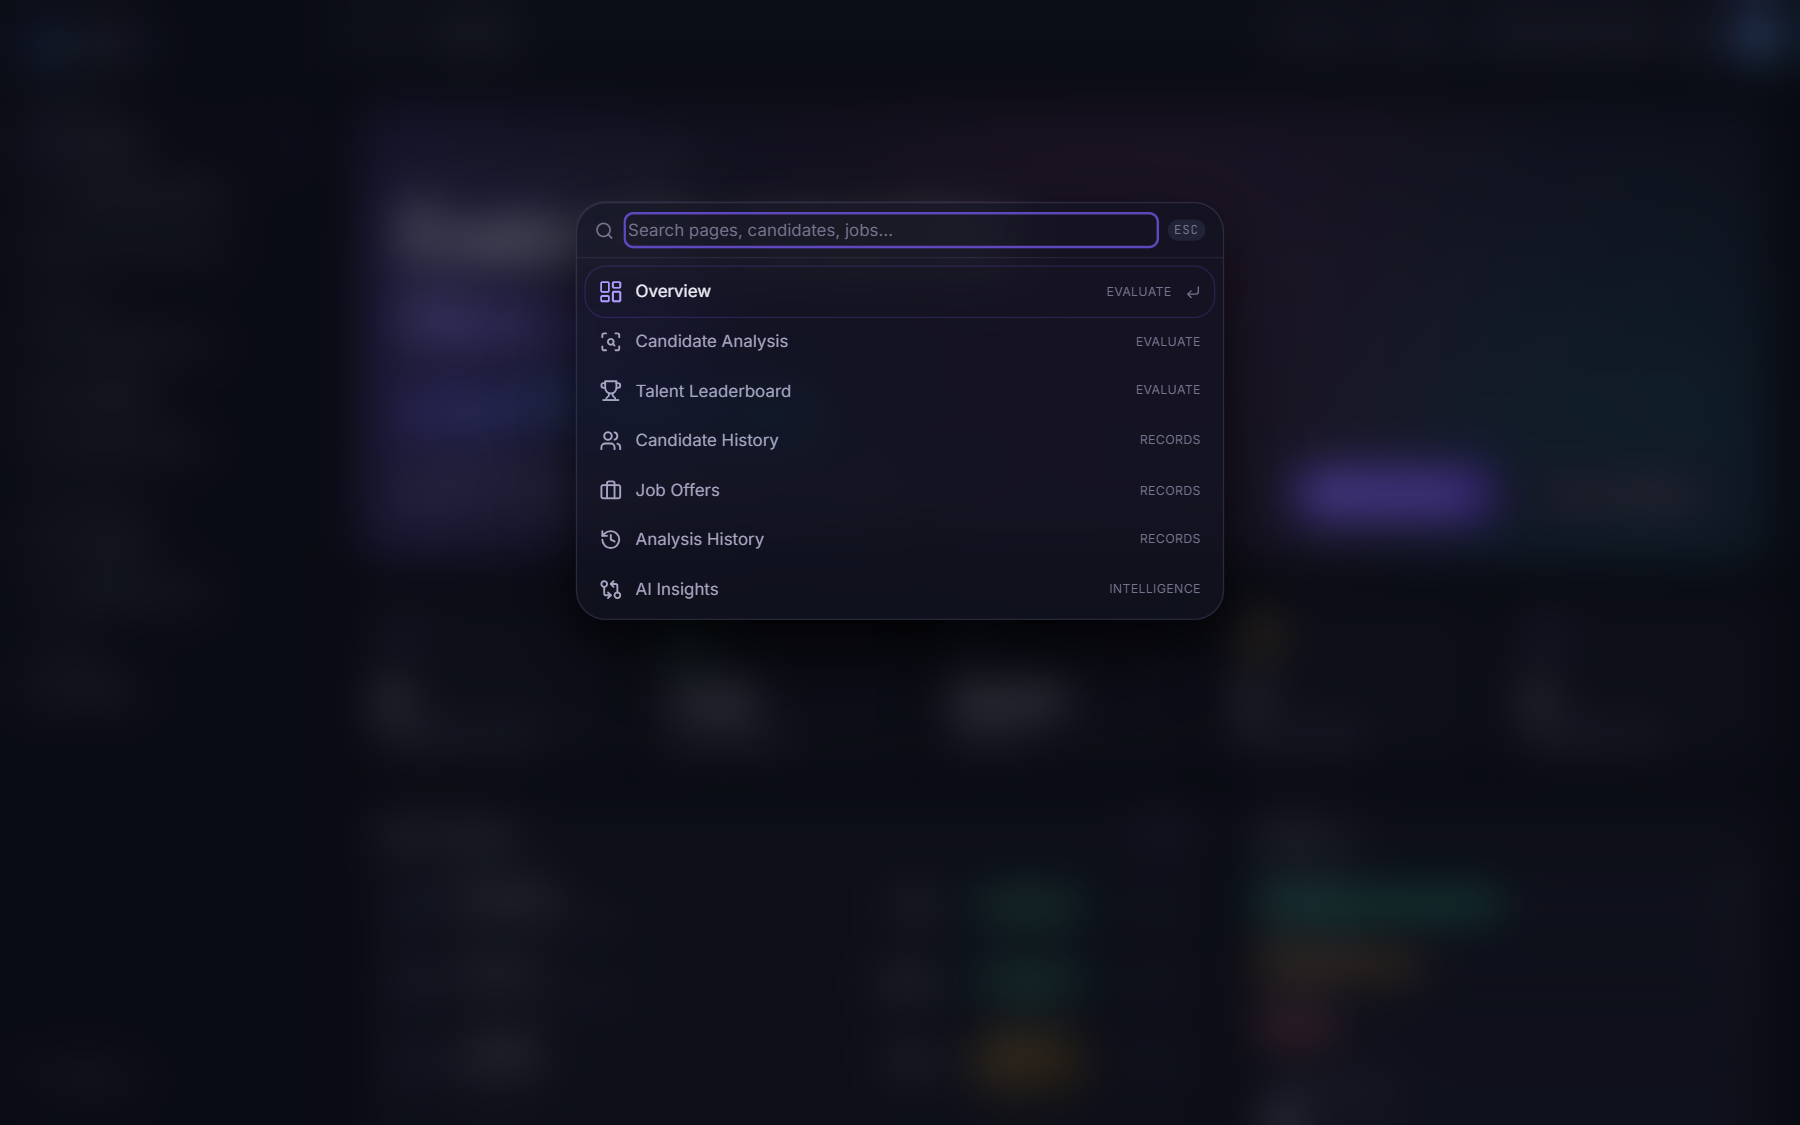
\includegraphics[width=.95\textwidth]{img/interfaces/search.png}
  \caption{Recherche transversale}
  \label{fig:chap5-search}
\end{figure}

La page \emph{Job Offers} permet de créer, consulter, modifier, fermer ou rouvrir une offre. Chaque offre possède un code, un titre, une description, des compétences demandées et un statut parmi \emph{OPEN}, \emph{ON\_HOLD} et \emph{CLOSED} (figures~\ref{fig:chap5-job-offers} et~\ref{fig:chap5-add-job-offer}).

\begin{figure}[H]
  \centering
  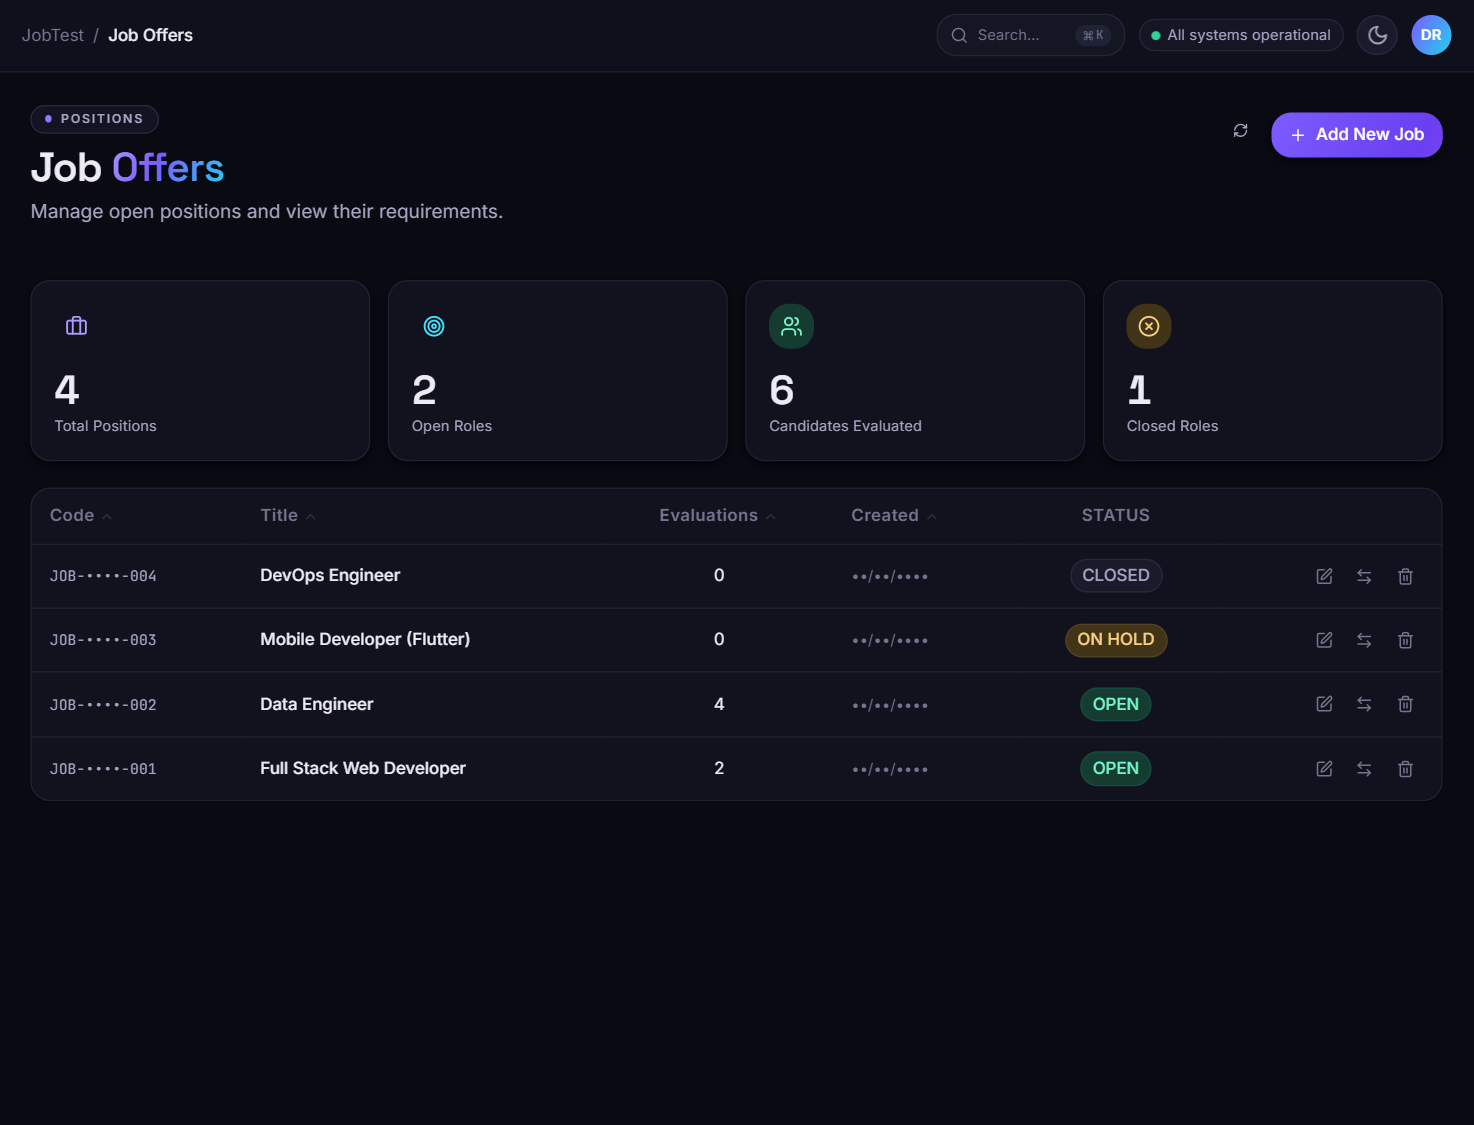
\includegraphics[width=.8\textwidth]{img/interfaces/job_offers.png}
  \caption{Liste des offres d'emploi}
  \label{fig:chap5-job-offers}
\end{figure}

\begin{figure}[H]
  \centering
  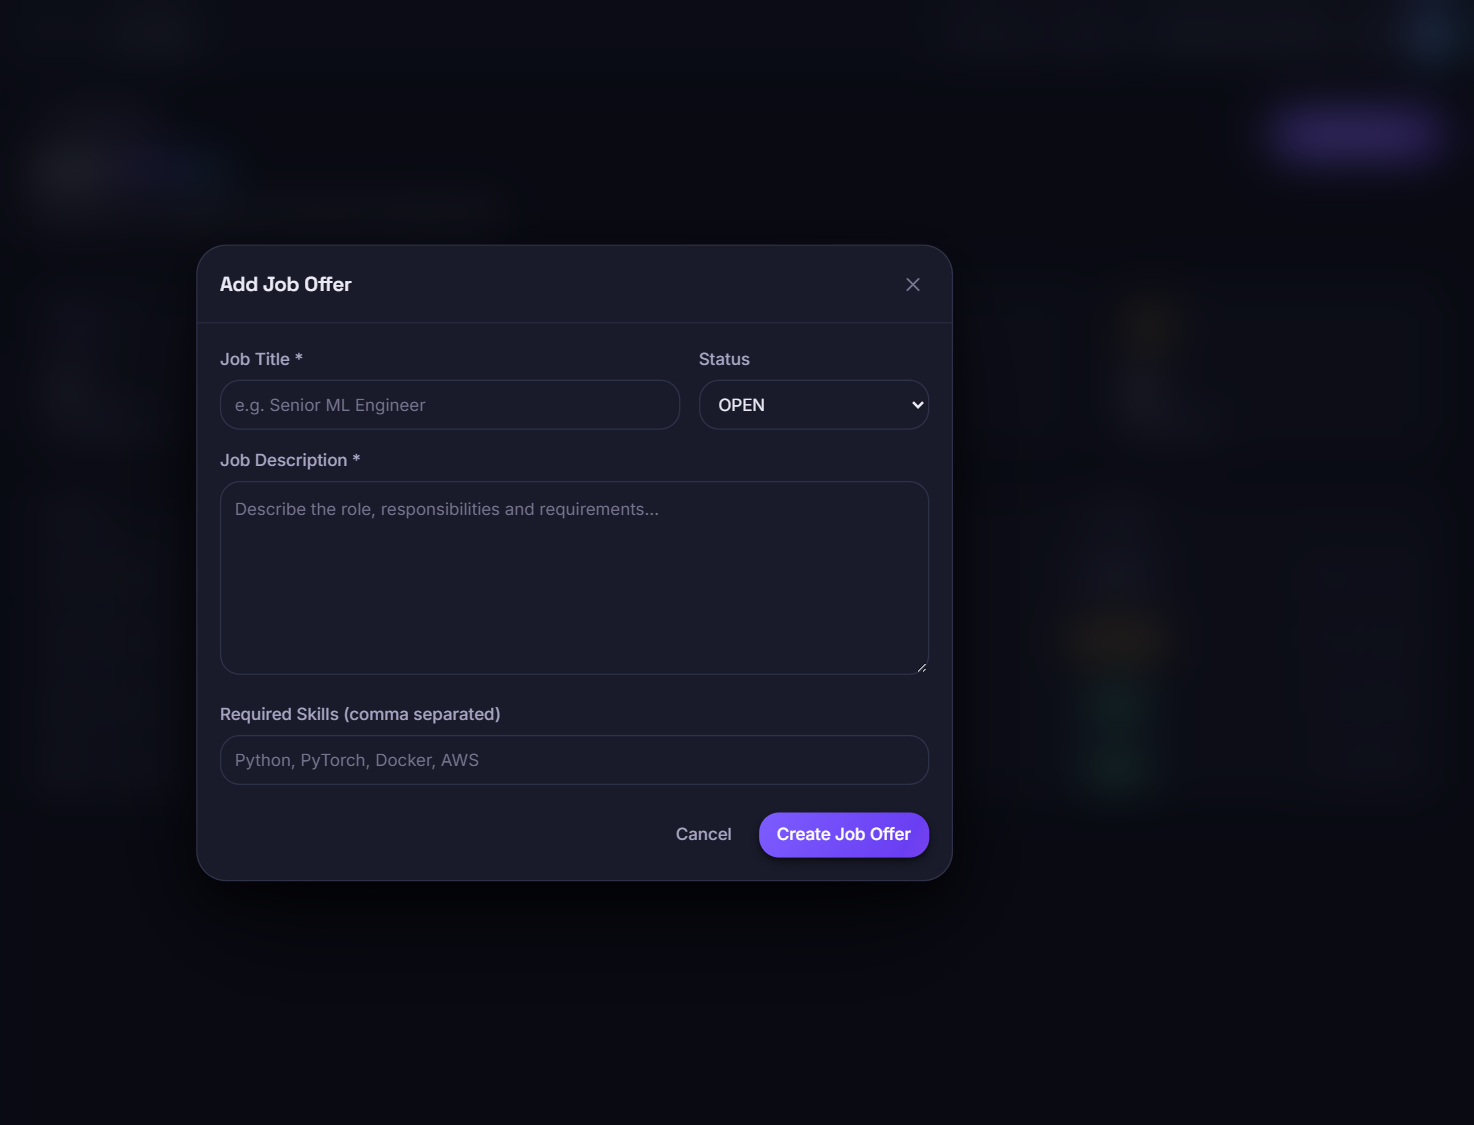
\includegraphics[width=.8\textwidth]{img/interfaces/add_job_offer.png}
  \caption{Création d'une offre d'emploi}
  \label{fig:chap5-add-job-offer}
\end{figure}

La page \emph{Candidate History} distingue les candidats des comptes recruteurs. Elle affiche les informations disponibles, l'état du parcours, le nombre d'évaluations et le meilleur score calibré de chaque candidat~; la modification et la suppression sont des actions explicites (figure~\ref{fig:chap5-candidate-history}).

\begin{figure}[H]
  \centering
  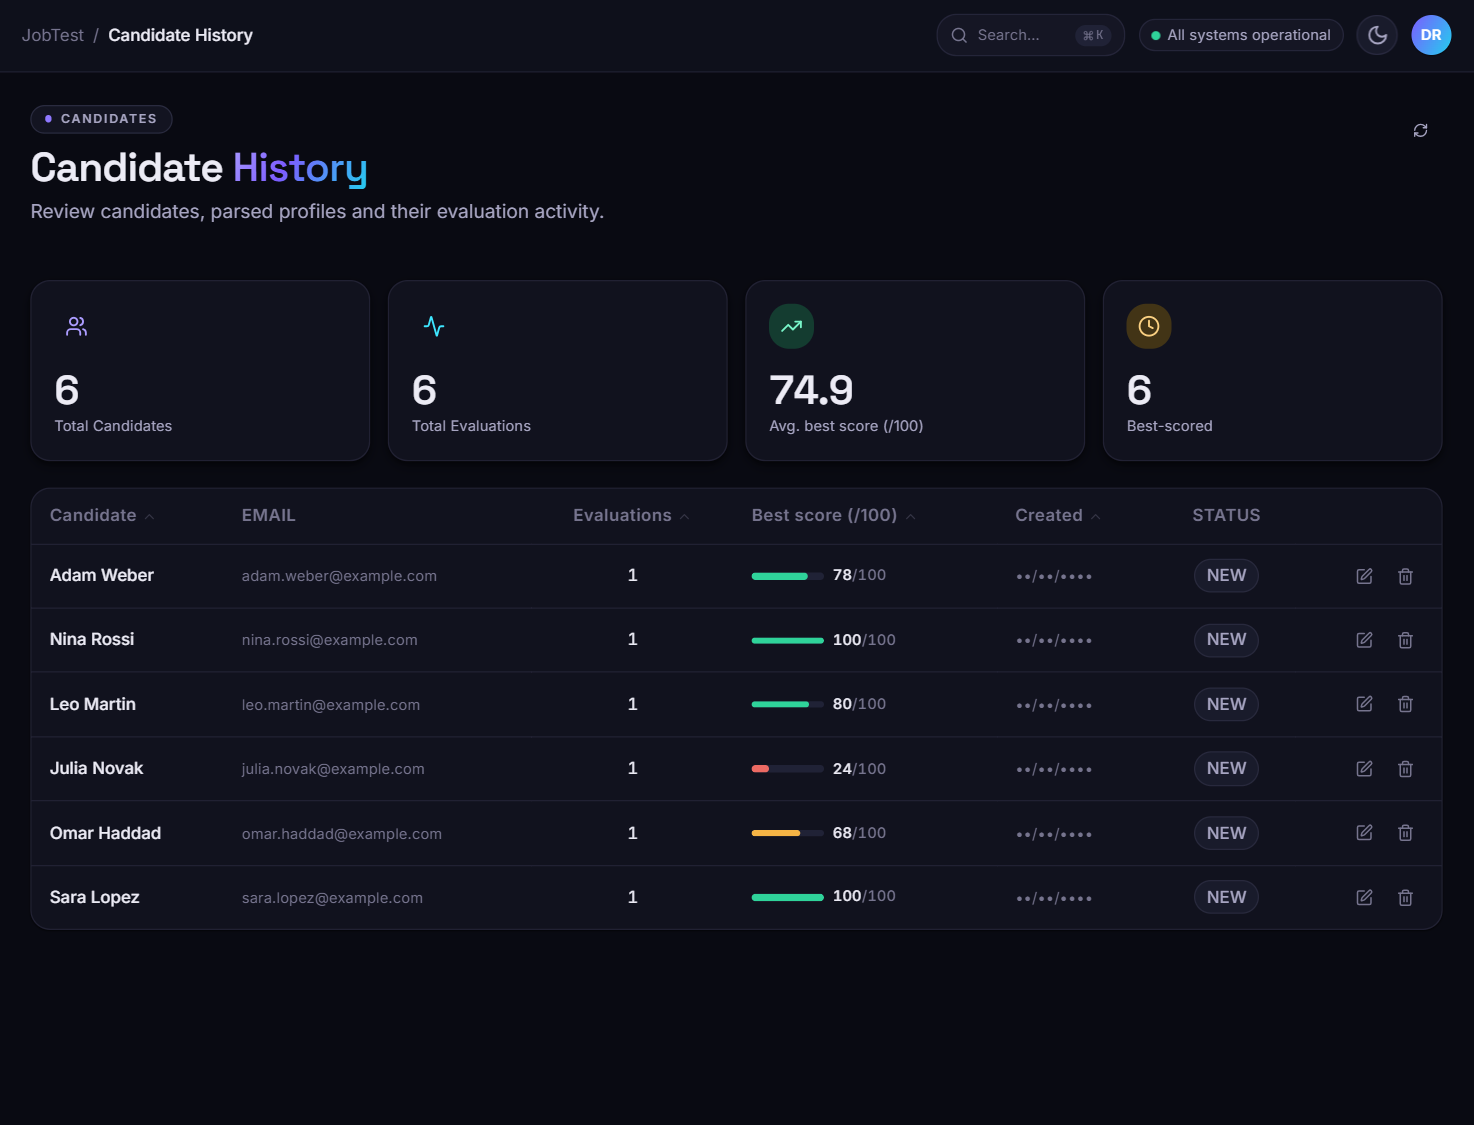
\includegraphics[width=.8\textwidth]{img/interfaces/condidate_history.png}
  \caption{Suivi des candidats}
  \label{fig:chap5-candidate-history}
\end{figure}

L'historique des évaluations liste chaque résultat persisté avec son offre, son score sur 100 et son verdict. Le panneau de détail rappelle la version de calibration, le score brut de la méthode et les seuils appliqués lors du calcul~; un résultat calculé sur l'ancienne échelle y serait signalé comme tel (figure~\ref{fig:chap5-analysis-history}).

\begin{figure}[H]
  \centering
  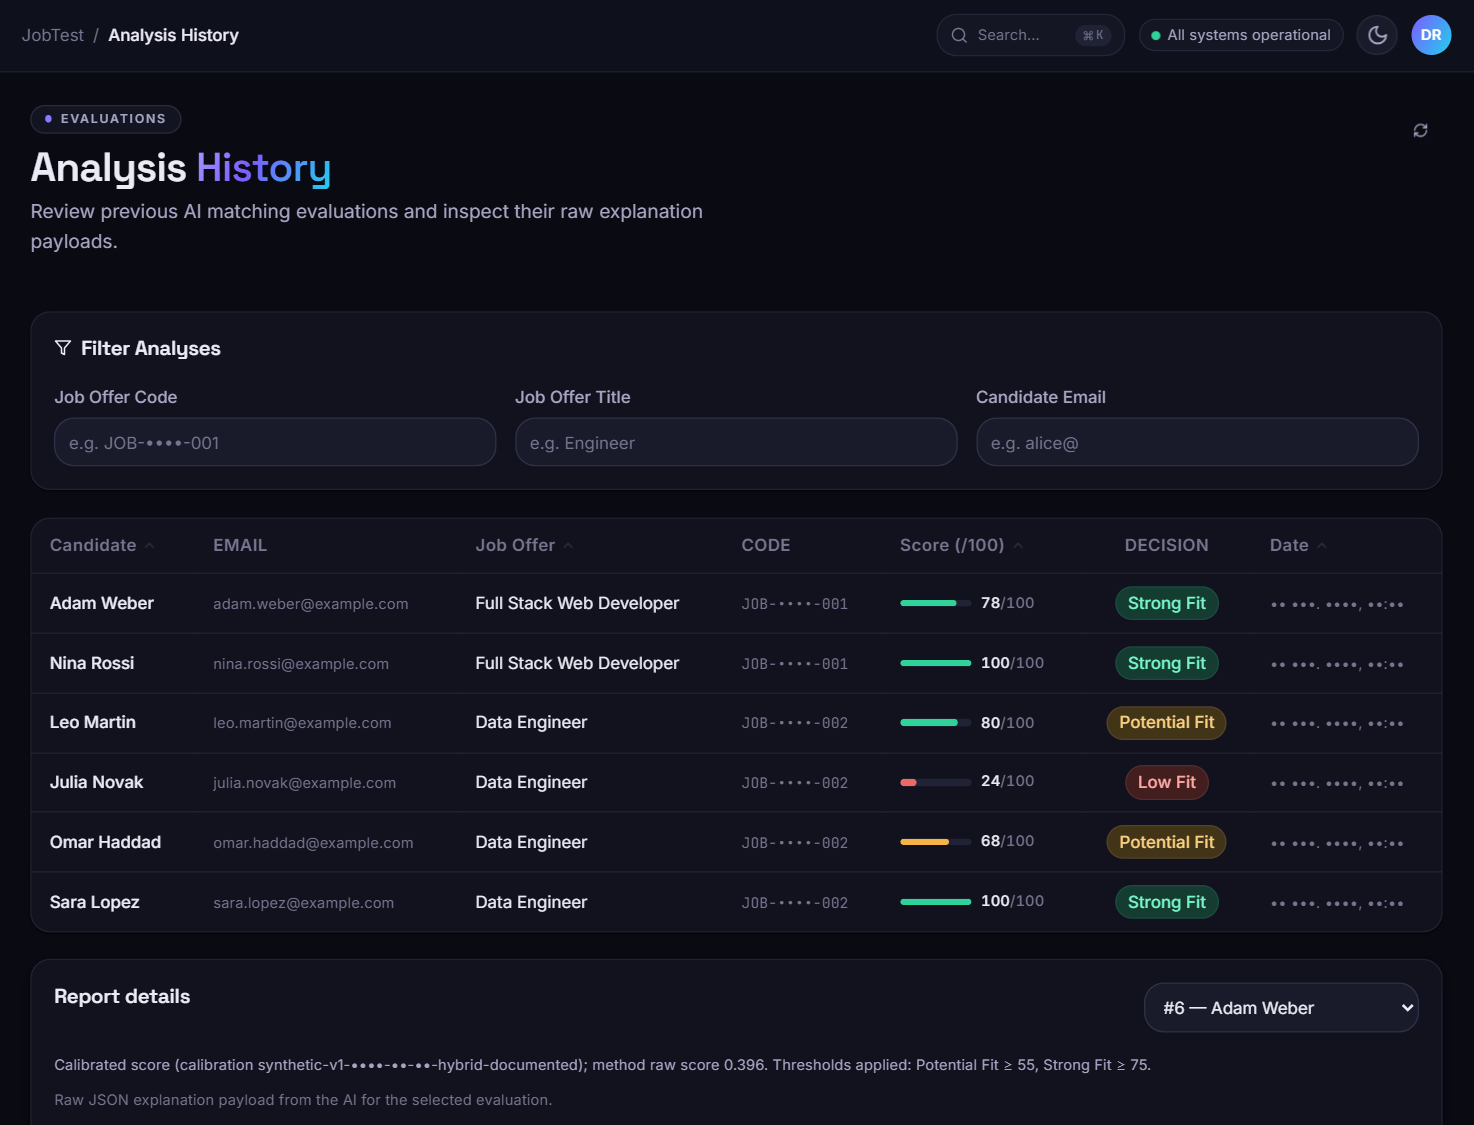
\includegraphics[width=.8\textwidth]{img/interfaces/analysis_history.png}
  \caption{Historique des évaluations}
  \label{fig:chap5-analysis-history}
\end{figure}

\subsection{Évaluation, résultat et analyse approfondie}

L'écran \emph{Candidate Analysis} constitue le point de départ du parcours principal. Il présente les compétences demandées par l'offre choisie, la politique de décision active et le bouton de lancement (figure~\ref{fig:chap5-analysis-entry}). L'exemple suivant évalue un CV fictif de développeur web face à l'offre \emph{Full Stack Web Developer}.

\begin{figure}[H]
  \centering
  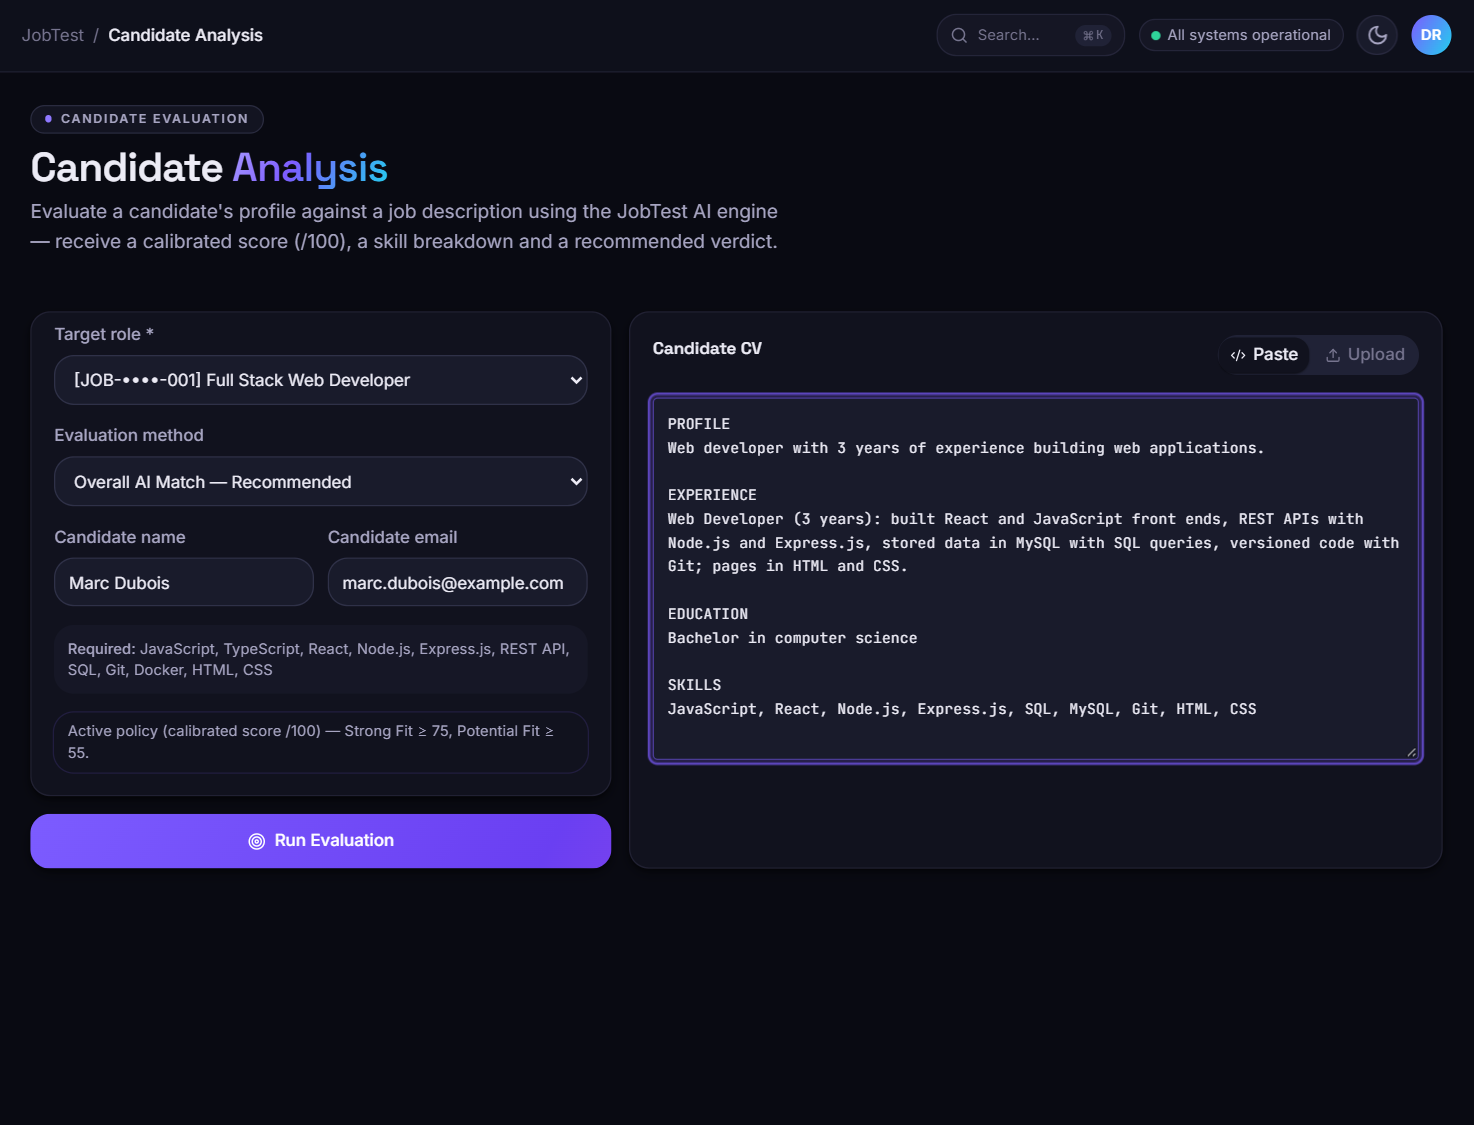
\includegraphics[width=.8\textwidth]{img/interfaces/condidate_anal_1.png}
  \caption{Saisie d'une évaluation}
  \label{fig:chap5-analysis-entry}
\end{figure}

Le résultat affiche le score calibré sur 100, le verdict recommandé, la distance au seuil le plus proche et la justification. Sous le score, une mention rappelle la version de calibration, le score brut de la méthode et les bandes appliquées. Dans cet exemple, le score brut de 0,651 dépasse la borne haute de la calibration (0,613)~: le score affiché atteint donc 100, alors que 8 des 11 compétences demandées sont reconnues. La justification signale aussi qu'une compétence exigée, TypeScript, reste à vérifier. La distance au seuil n'est pas une probabilité (figure~\ref{fig:chap5-analysis-score}).

\begin{figure}[H]
  \centering
  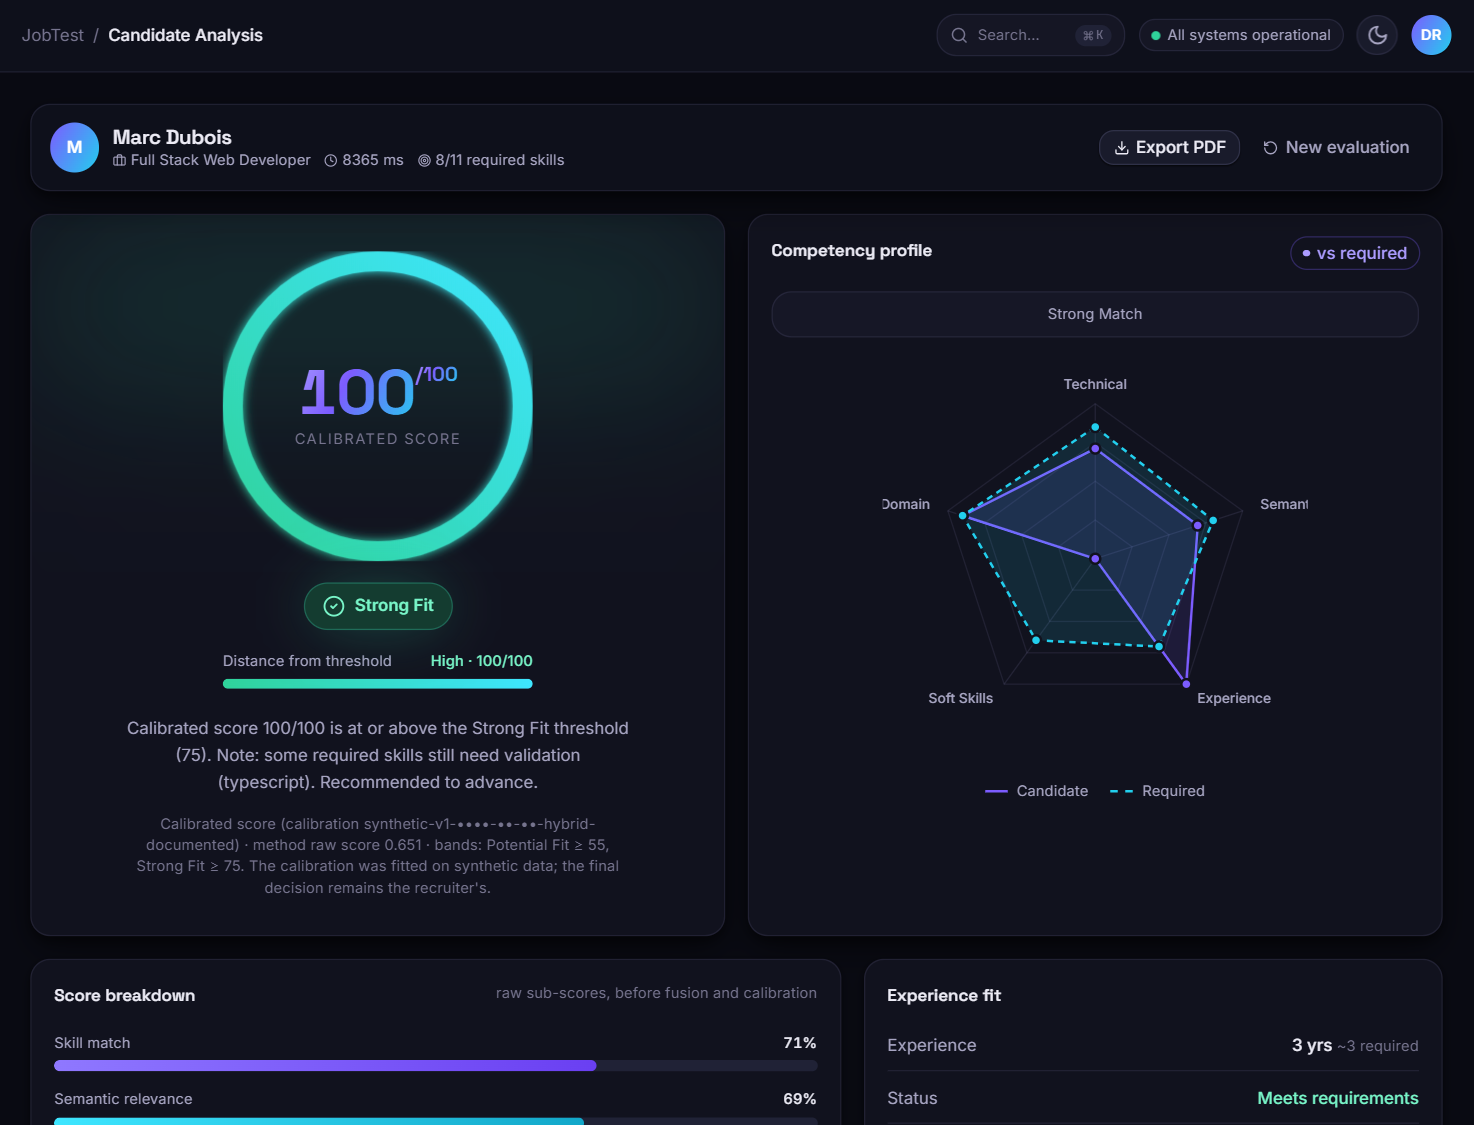
\includegraphics[width=.8\textwidth]{img/interfaces/condidate_anal_2.png}
  \caption{Score, verdict et profil de compétences}
  \label{fig:chap5-analysis-score}
\end{figure}

Les sous-scores sont présentés comme des valeurs brutes, avant fusion et calibration, à côté de l'adéquation d'expérience (figure~\ref{fig:chap5-analysis-components}). Les onglets donnent accès aux compétences, aux forces et écarts, aux actions recommandées et aux données brutes.

\begin{figure}[H]
  \centering
  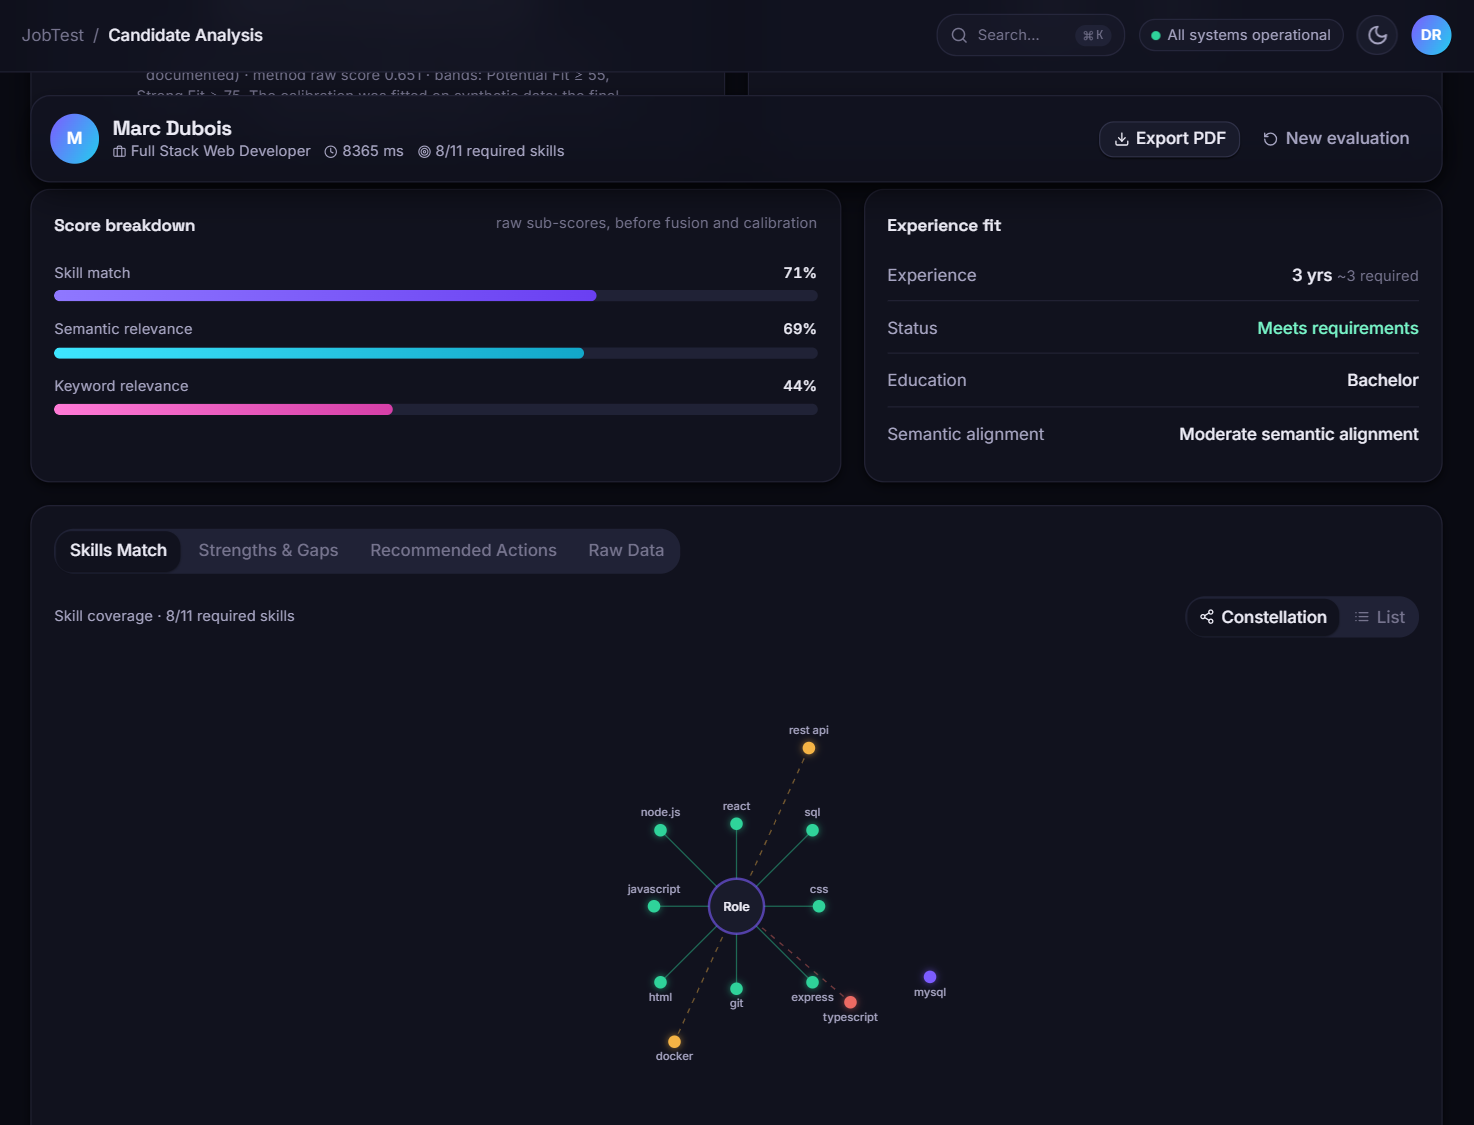
\includegraphics[width=.8\textwidth]{img/interfaces/condidate_anal_3.png}
  \caption{Sous-scores et adéquation d'expérience}
  \label{fig:chap5-analysis-components}
\end{figure}

La constellation des compétences distingue les compétences reconnues, les lacunes prioritaires, les compétences manquantes et les compétences supplémentaires du candidat (figure~\ref{fig:chap5-analysis-visualization}).

\begin{figure}[H]
  \centering
  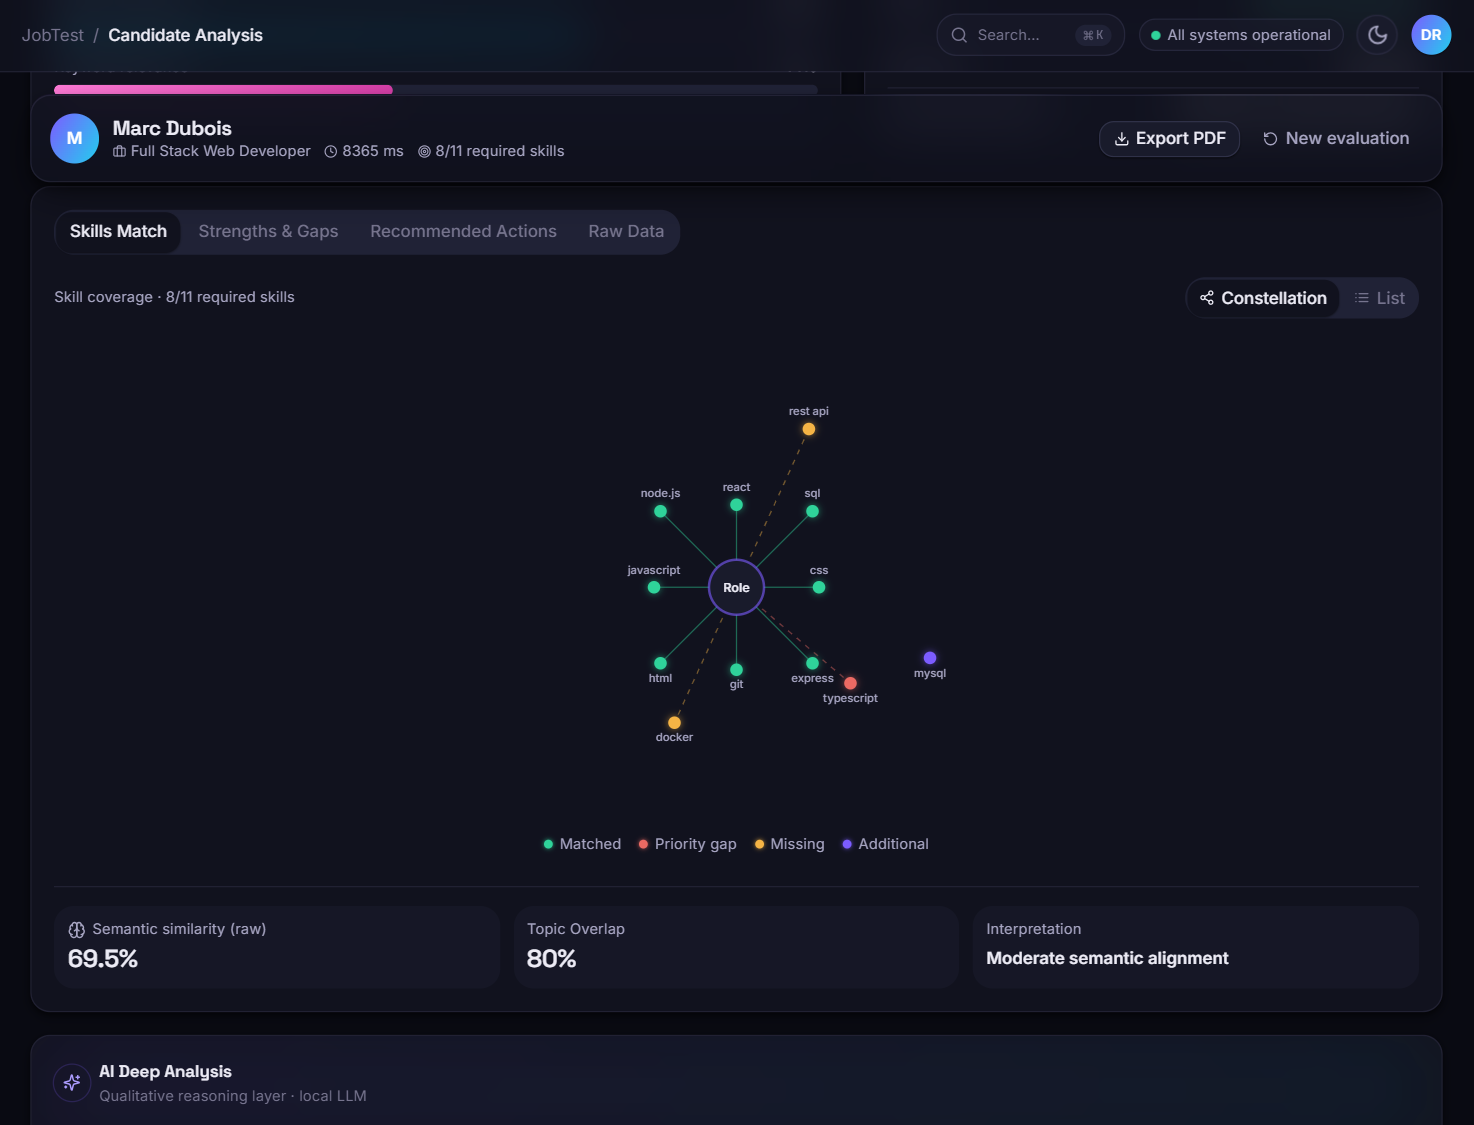
\includegraphics[width=.8\textwidth]{img/interfaces/condidate_anal_4.png}
  \caption{Compétences reconnues et manquantes}
  \label{fig:chap5-analysis-visualization}
\end{figure}

L'analyse approfondie est demandée automatiquement après l'affichage du résultat. Exécutée localement par \texttt{qwen2.5:1.5b} via Ollama, elle propose une synthèse, une trajectoire, des signaux à examiner, des recommandations et des questions d'entretien. Une mention rappelle qu'elle ne modifie ni le score ni le verdict (figure~\ref{fig:chap5-analysis-deep}). Si le runtime ne répond pas, son indisponibilité est affichée sans altérer le résultat principal.

\begin{figure}[H]
  \centering
  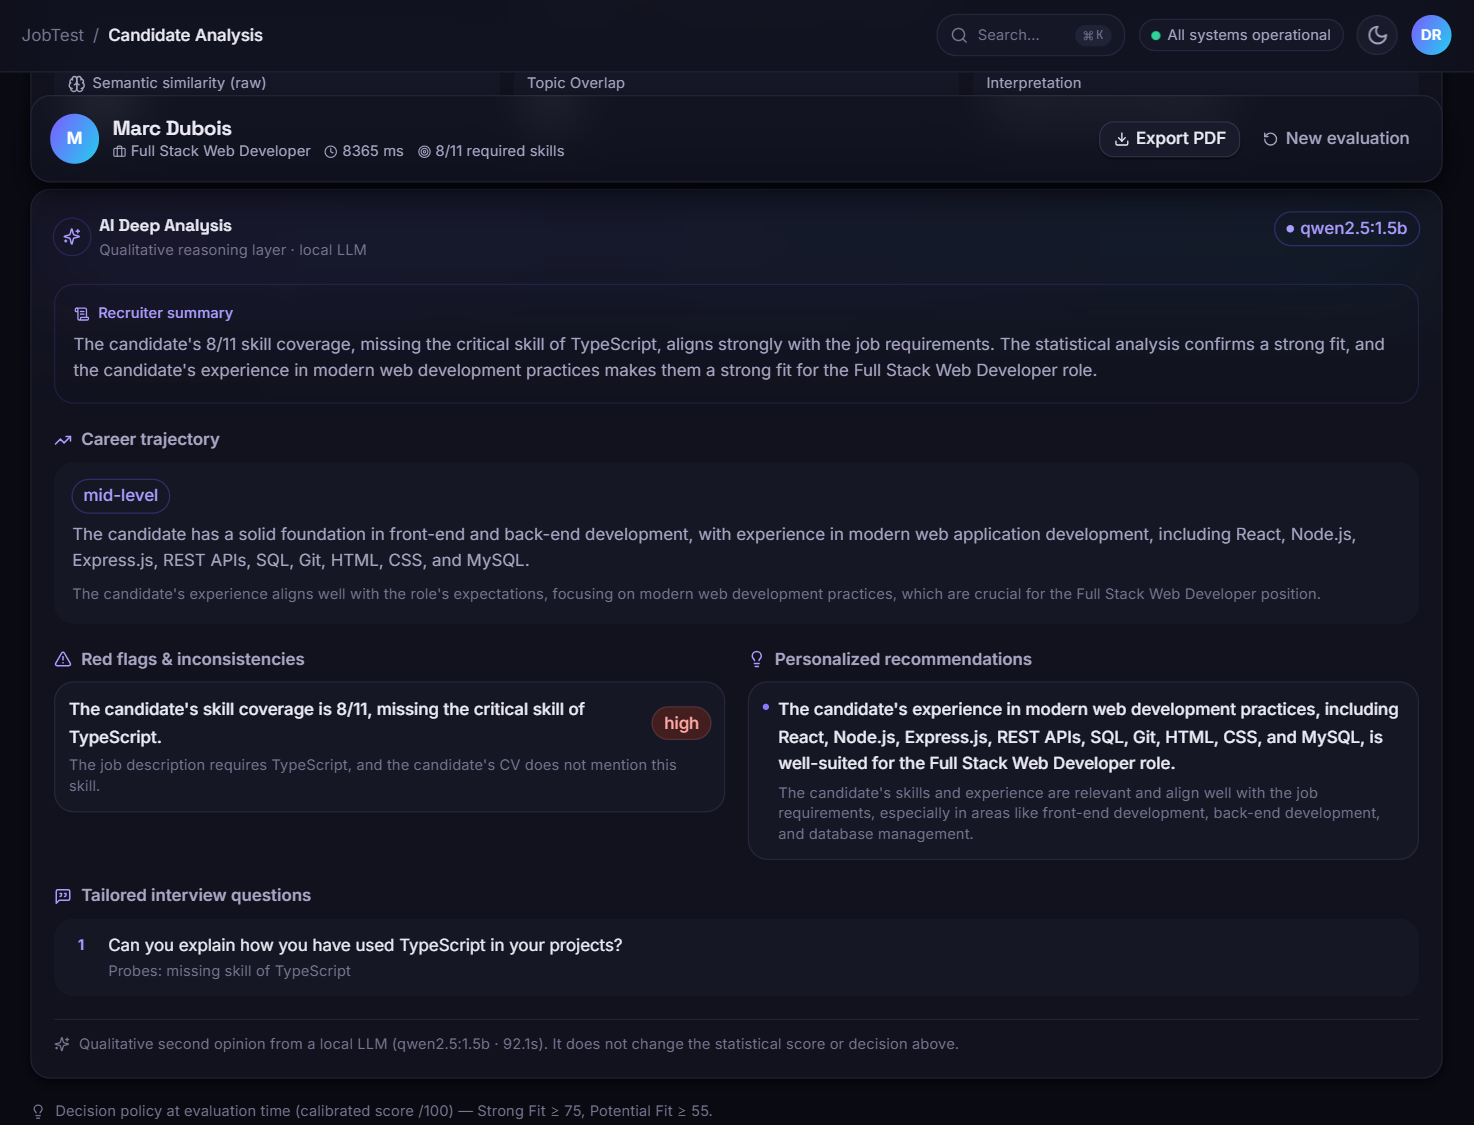
\includegraphics[width=.8\textwidth]{img/interfaces/condidate_anal_5.png}
  \caption{Analyse approfondie locale}
  \label{fig:chap5-analysis-deep}
\end{figure}

Lorsque les compétences correspondantes reposent surtout sur des déclarations ou sur du texte recopié de l'offre, un encadré \emph{Evidence check} le signale. La figure~\ref{fig:chap5-evidence} montre un CV fictif de graphiste complété par la liste des compétences de l'offre \emph{Data Engineer}~: son score calibré atteint 80,6, mais aucune des huit compétences correspondantes n'apparaît dans l'expérience décrite. Le verdict est donc limité à \emph{Potential Fit} (\texttt{CONSIDER}), avec la liste des compétences seulement déclarées.

\begin{figure}[H]
  \centering
  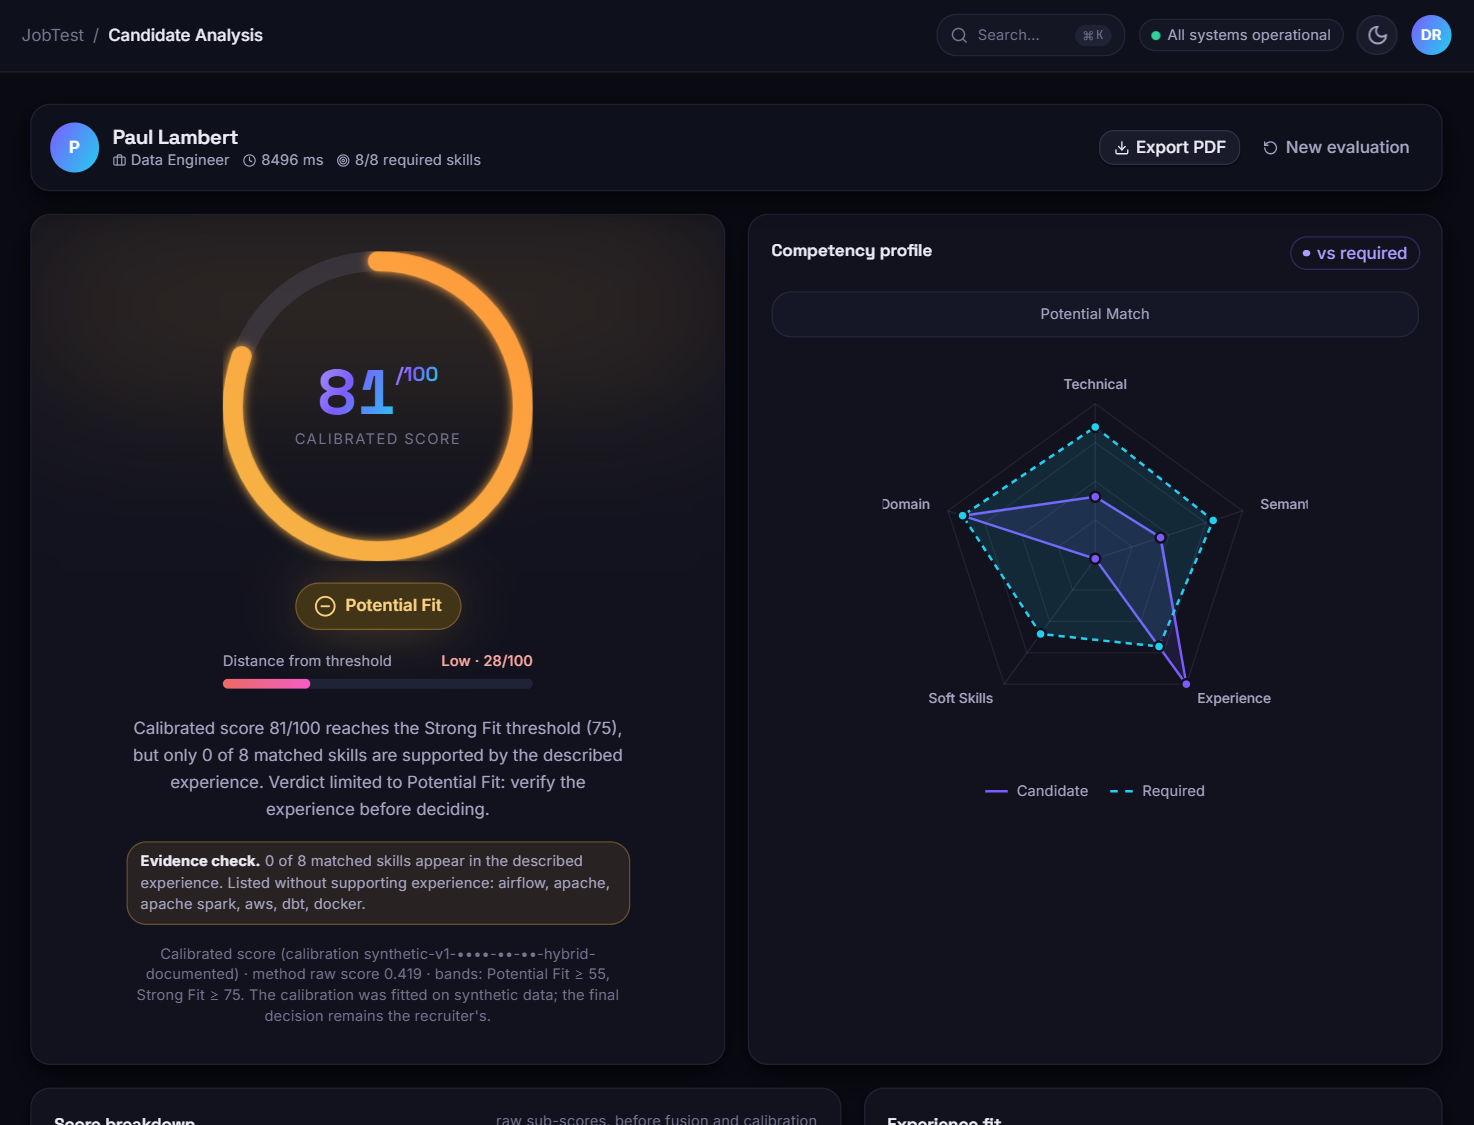
\includegraphics[width=.8\textwidth]{img/interfaces/evidence_check.png}
  \caption{Verdict limité par le contrôle des preuves}
  \label{fig:chap5-evidence}
\end{figure}

\subsection{Classement, comparaison, qualité et paramètres}

Le \emph{Talent Leaderboard} accepte plusieurs CV pour une offre et restitue un classement. Les figures~\ref{fig:chap5-leaderboard-selection} à~\ref{fig:chap5-leaderboard-result} rejouent avec la version finale l'essai décrit au chapitre~\ref{chap:tests-securite}~: dix-huit CV fictifs au format PDF face à l'offre \emph{Full Stack Web Developer}. L'export CSV du classement inclut le score calibré, le score brut, les seuils et la version de calibration.

\begin{figure}[H]
  \centering
  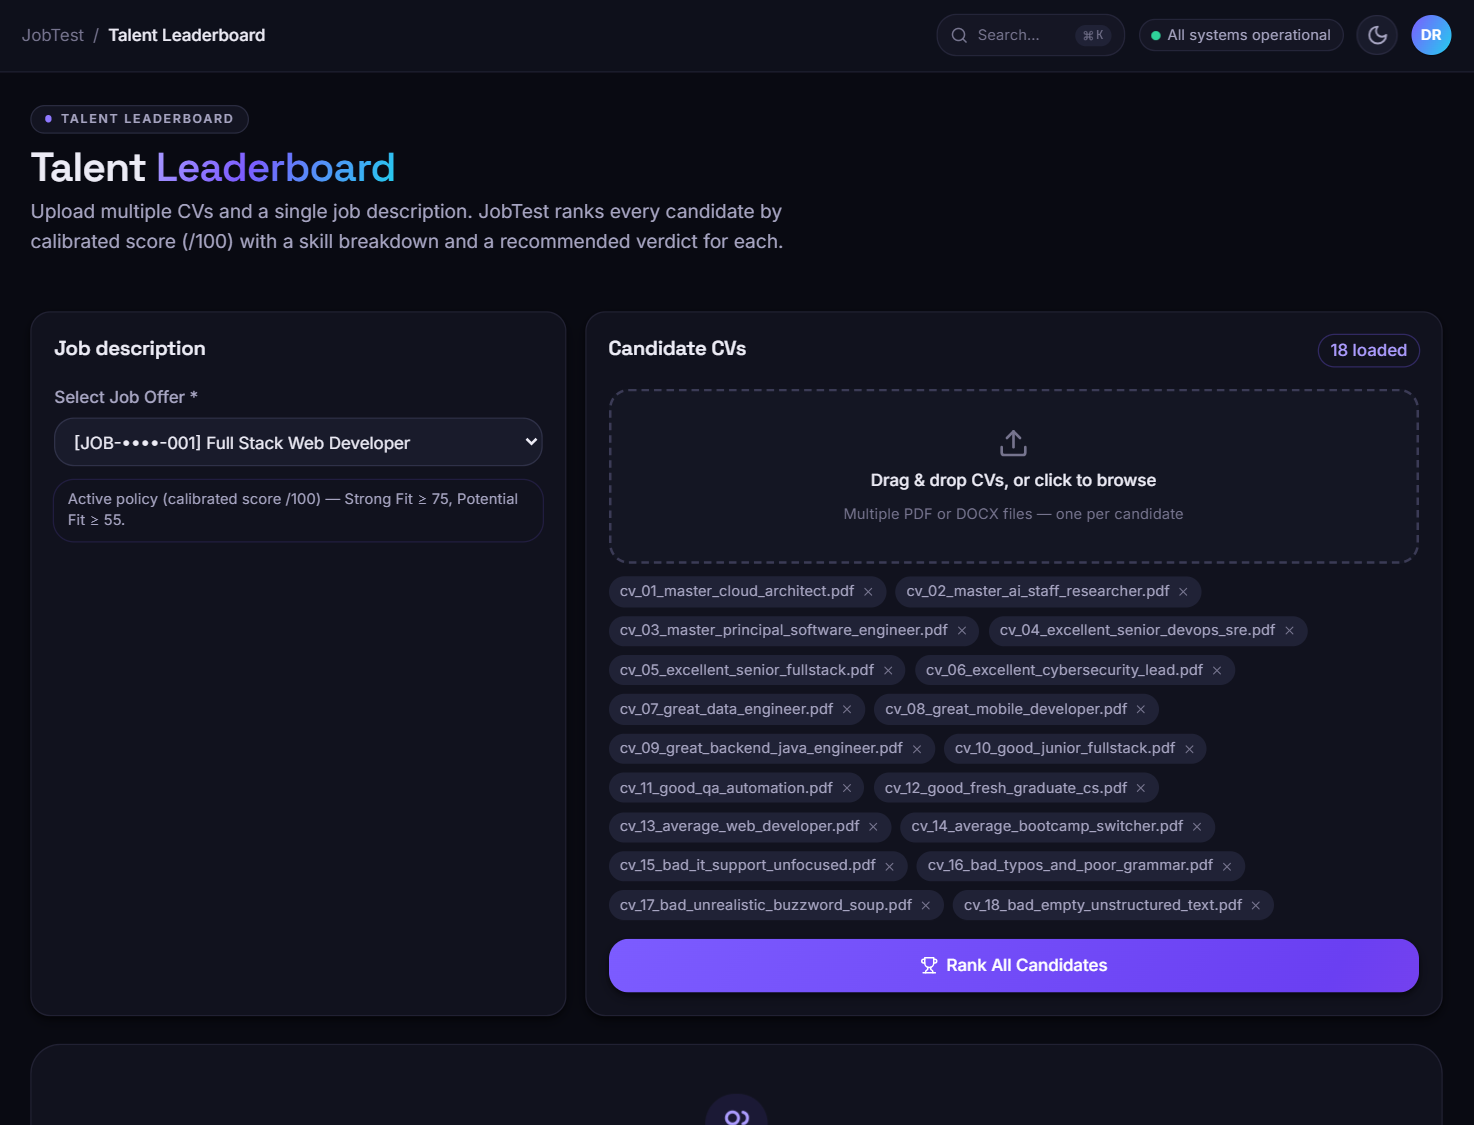
\includegraphics[width=.8\textwidth]{img/interfaces/talent_leader_1.png}
  \caption{Sélection de l'offre et des CV}
  \label{fig:chap5-leaderboard-selection}
\end{figure}

\begin{figure}[H]
  \centering
  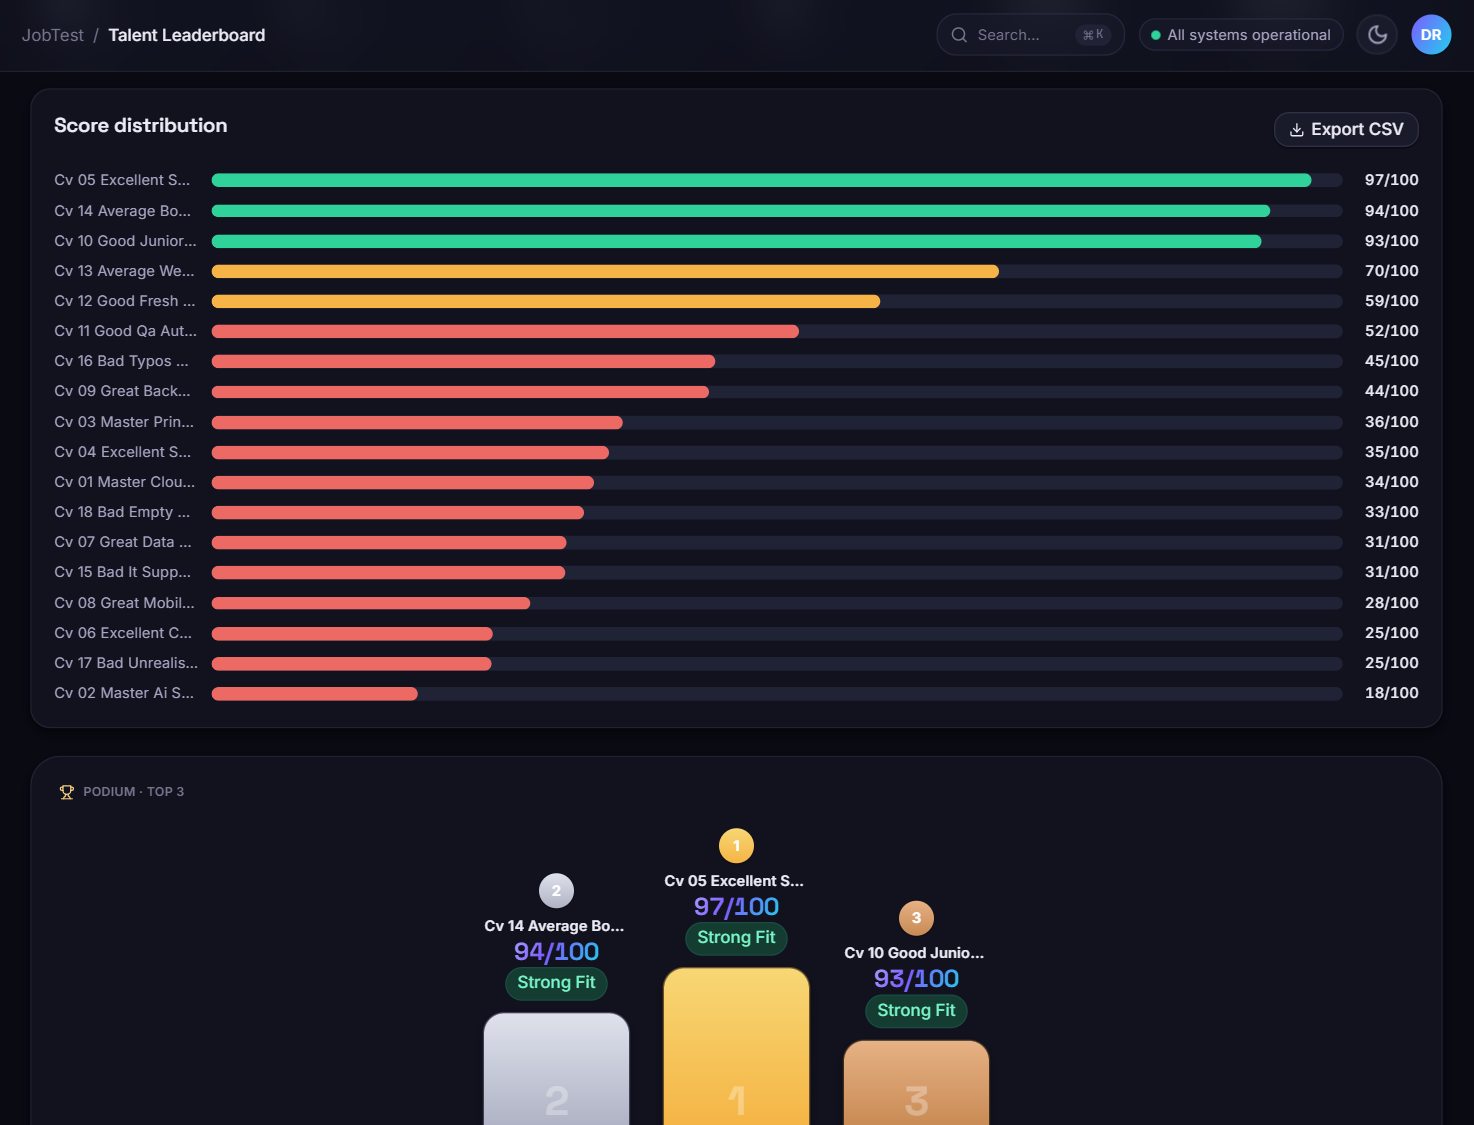
\includegraphics[width=.8\textwidth]{img/interfaces/talent_leader_2.png}
  \caption{Distribution des scores du classement}
  \label{fig:chap5-leaderboard-ranking}
\end{figure}

\begin{figure}[H]
  \centering
  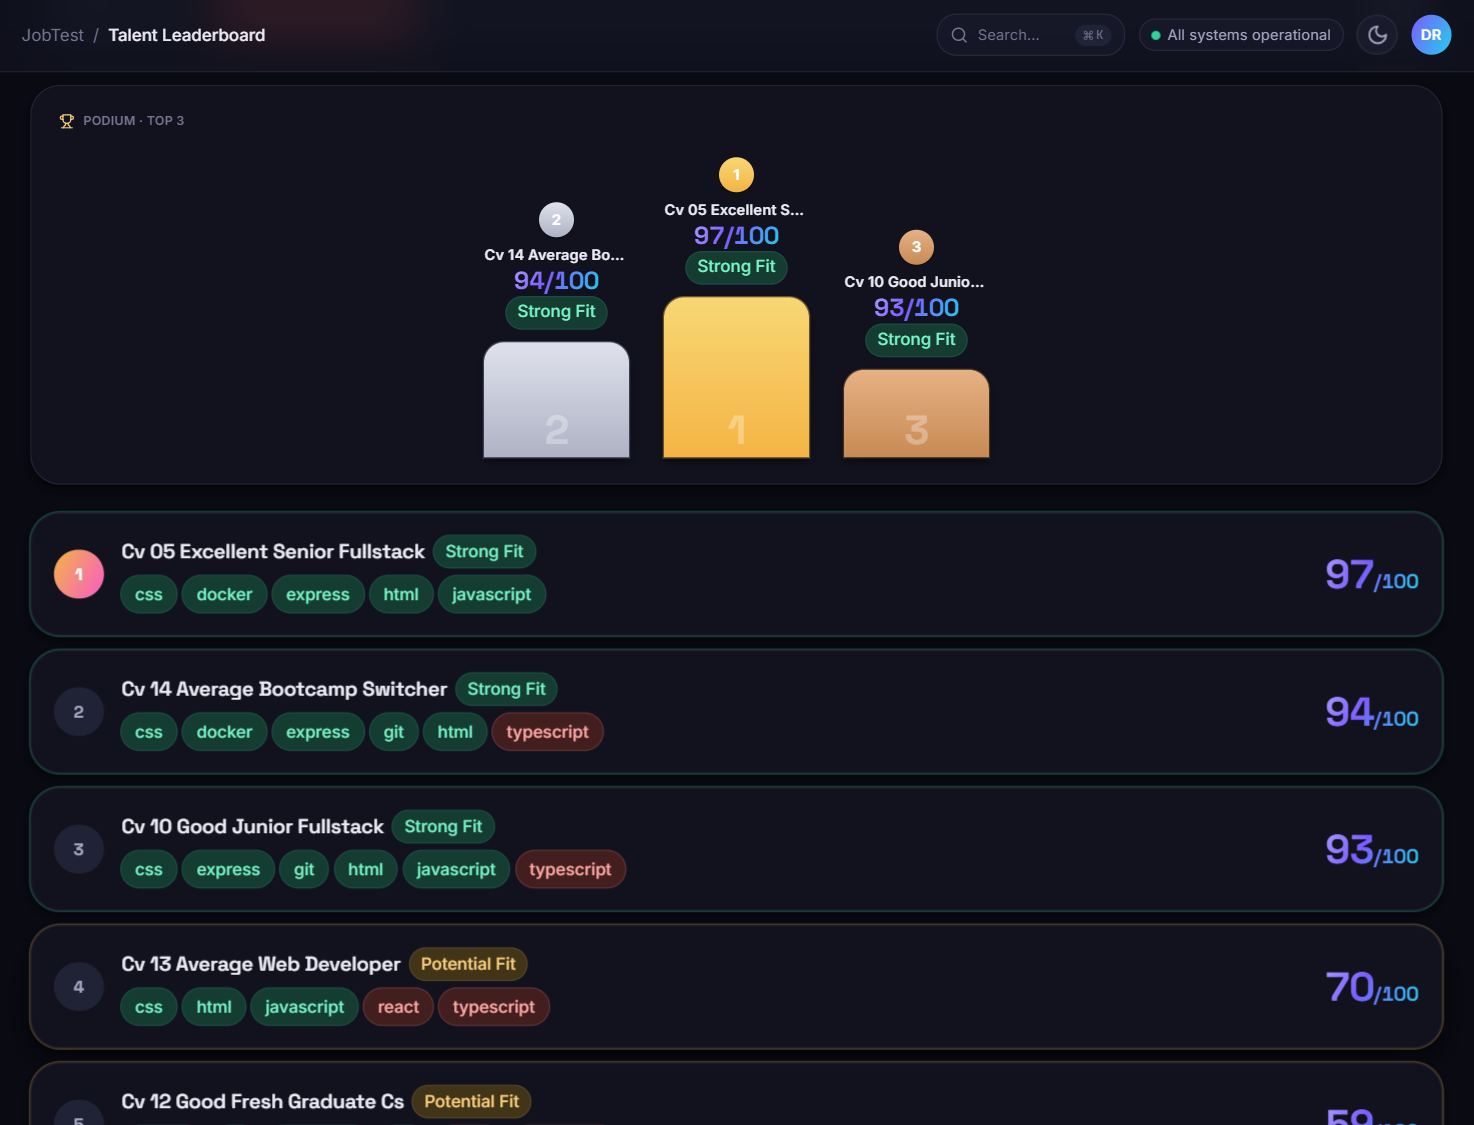
\includegraphics[width=.8\textwidth]{img/interfaces/talent_leader_3.png}
  \caption{Podium du classement}
  \label{fig:chap5-leaderboard-podium}
\end{figure}

\begin{figure}[H]
  \centering
  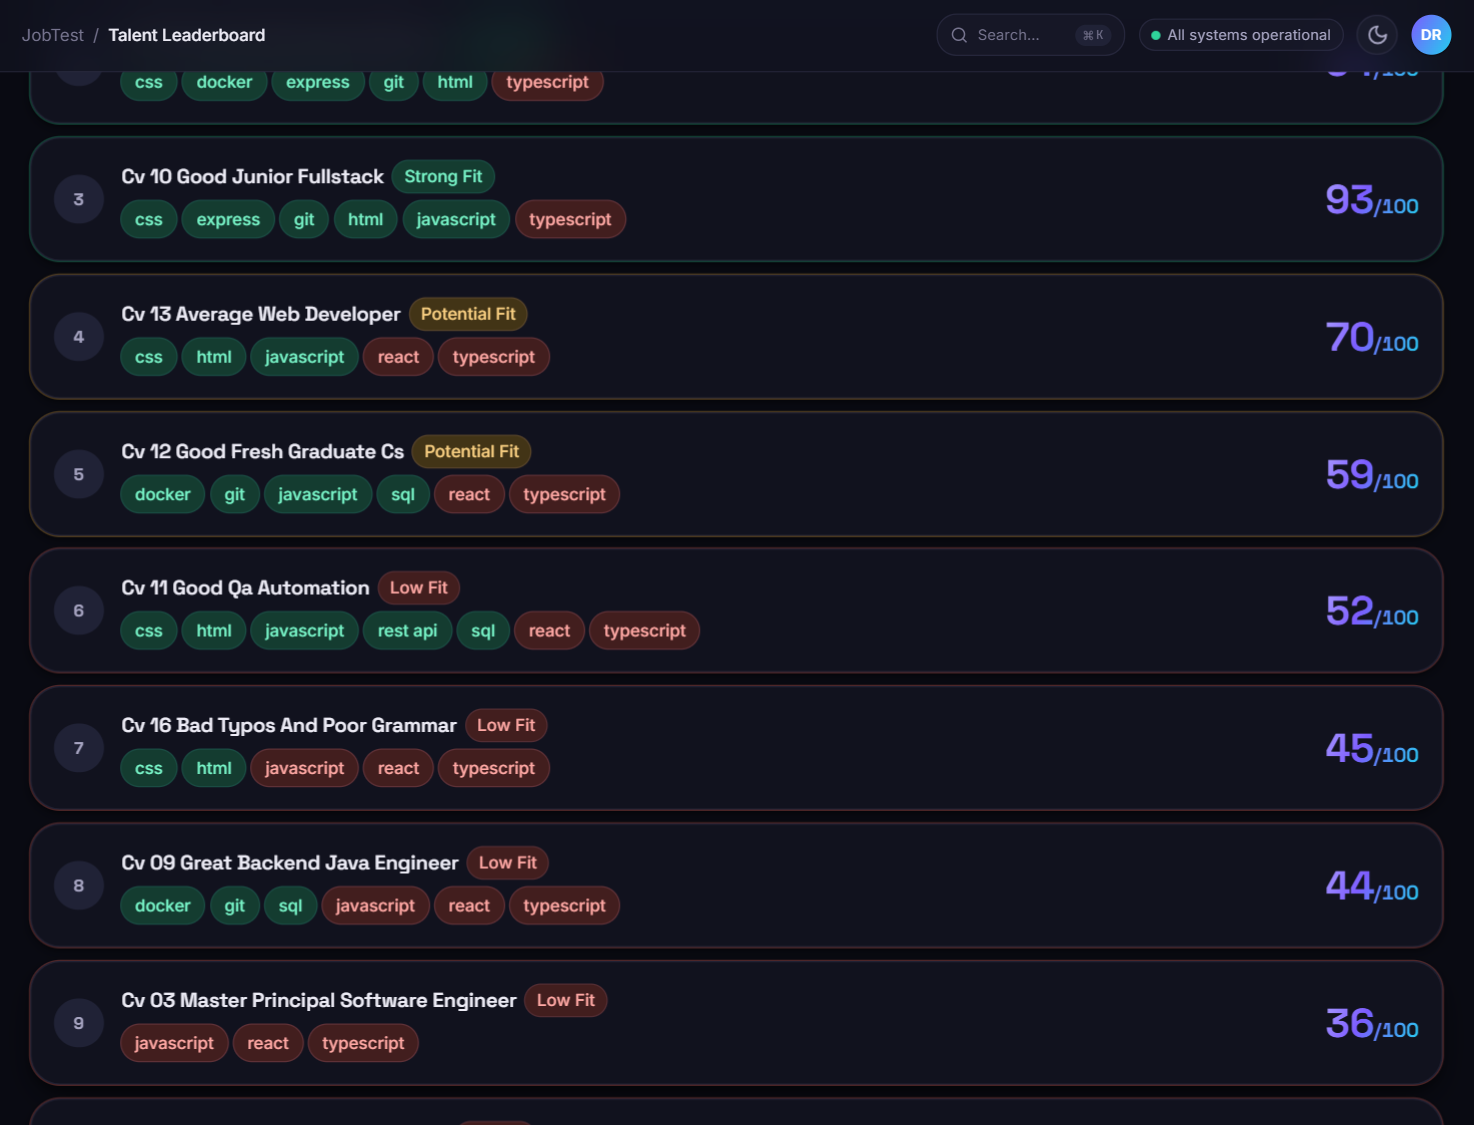
\includegraphics[width=.8\textwidth]{img/interfaces/talent_leader_4.png}
  \caption{Suite du classement}
  \label{fig:chap5-leaderboard-result}
\end{figure}

\emph{AI Insights} compare les quatre méthodes sur un même couple CV--offre sans créer de résultat persistant. Chaque score brut est ramené à l'échelle sur 100 par sa propre calibration, et les barres sont tracées sur cette échelle commune avec les bornes 55 et 75 (figure~\ref{fig:chap5-insights}).

\begin{figure}[H]
  \centering
  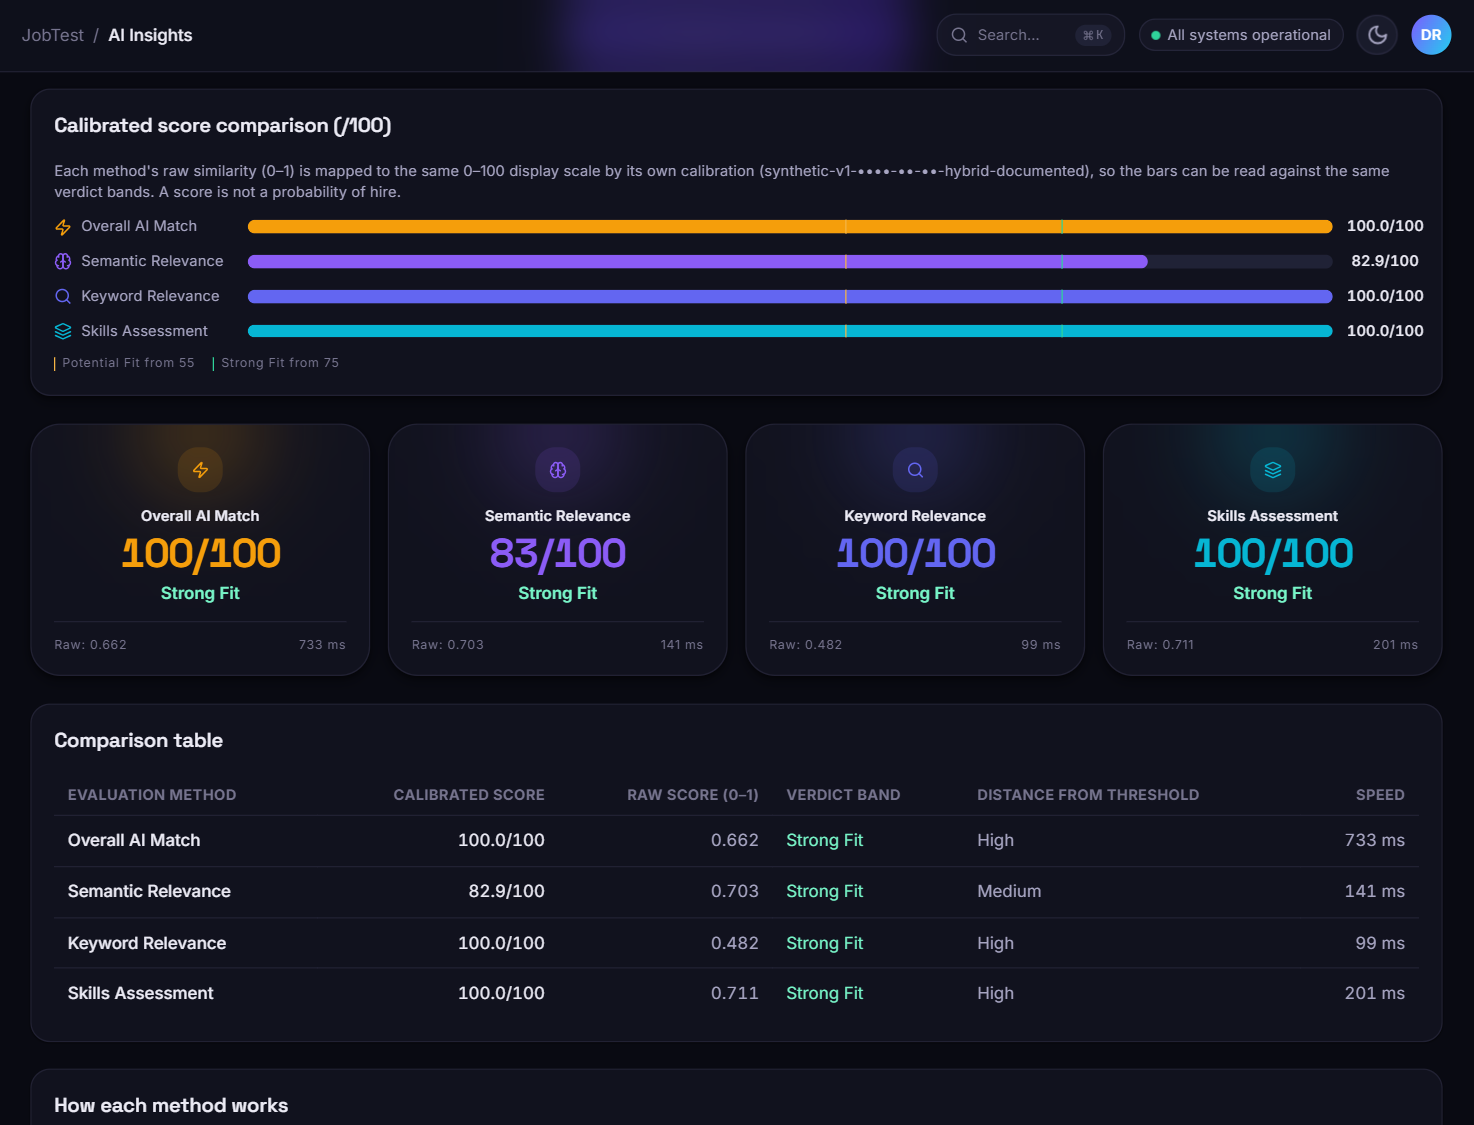
\includegraphics[width=.8\textwidth]{img/interfaces/insights.png}
  \caption{Comparaison des quatre méthodes}
  \label{fig:chap5-insights}
\end{figure}

L'écran de paramètres règle les seuils \emph{Strong Fit} et \emph{Potential Fit}, exprimés sur l'échelle calibrée, et présente l'état des composants de la plateforme (figure~\ref{fig:chap5-settings}).

\begin{figure}[H]
  \centering
  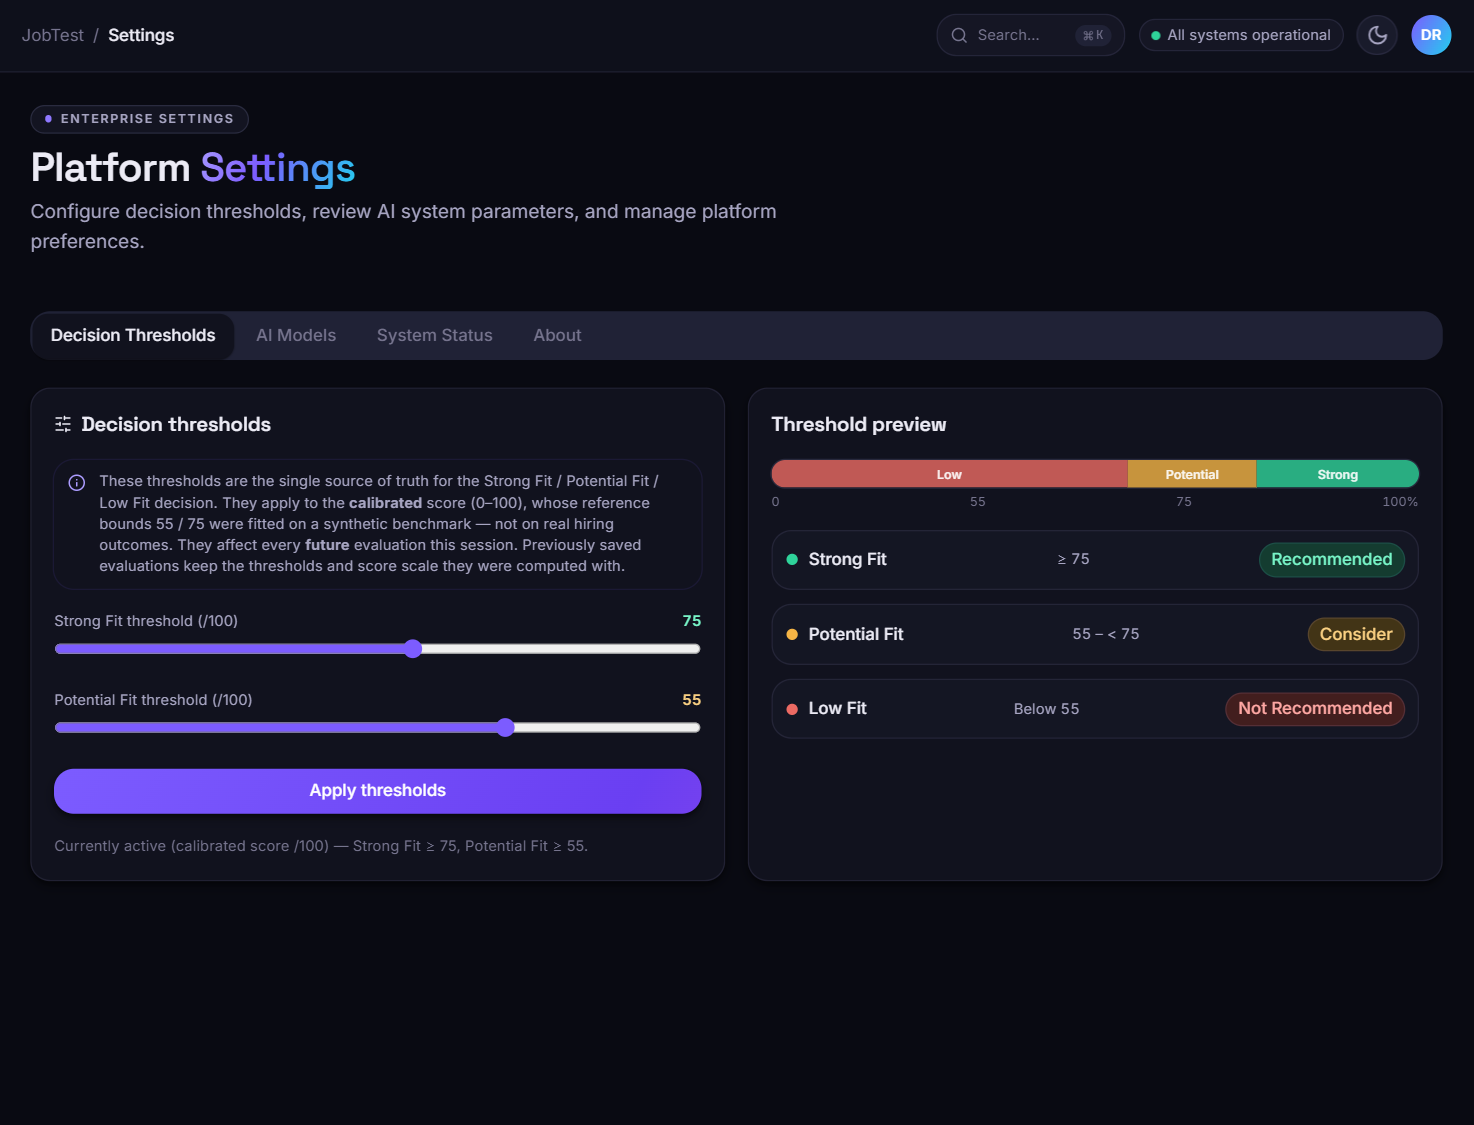
\includegraphics[width=.8\textwidth]{img/interfaces/plateform_settings.png}
  \caption{Réglage des seuils de décision}
  \label{fig:chap5-settings}
\end{figure}

L'écran \emph{AI Quality Center} présente les résultats d'évaluation hors ligne en indiquant pour chacun le fichier source, la taille de l'échantillon et sa concordance avec la calibration livrée. Il distingue trois catégories~: le banc d'essai synthétique, seul porteur de métriques~; les essais fonctionnels sur CV fictifs~; et les essais menés avec mes propres CV, pour lesquels les métriques sont affichées comme non mesurées (figure~\ref{fig:chap5-quality-1}).

\begin{figure}[H]
  \centering
  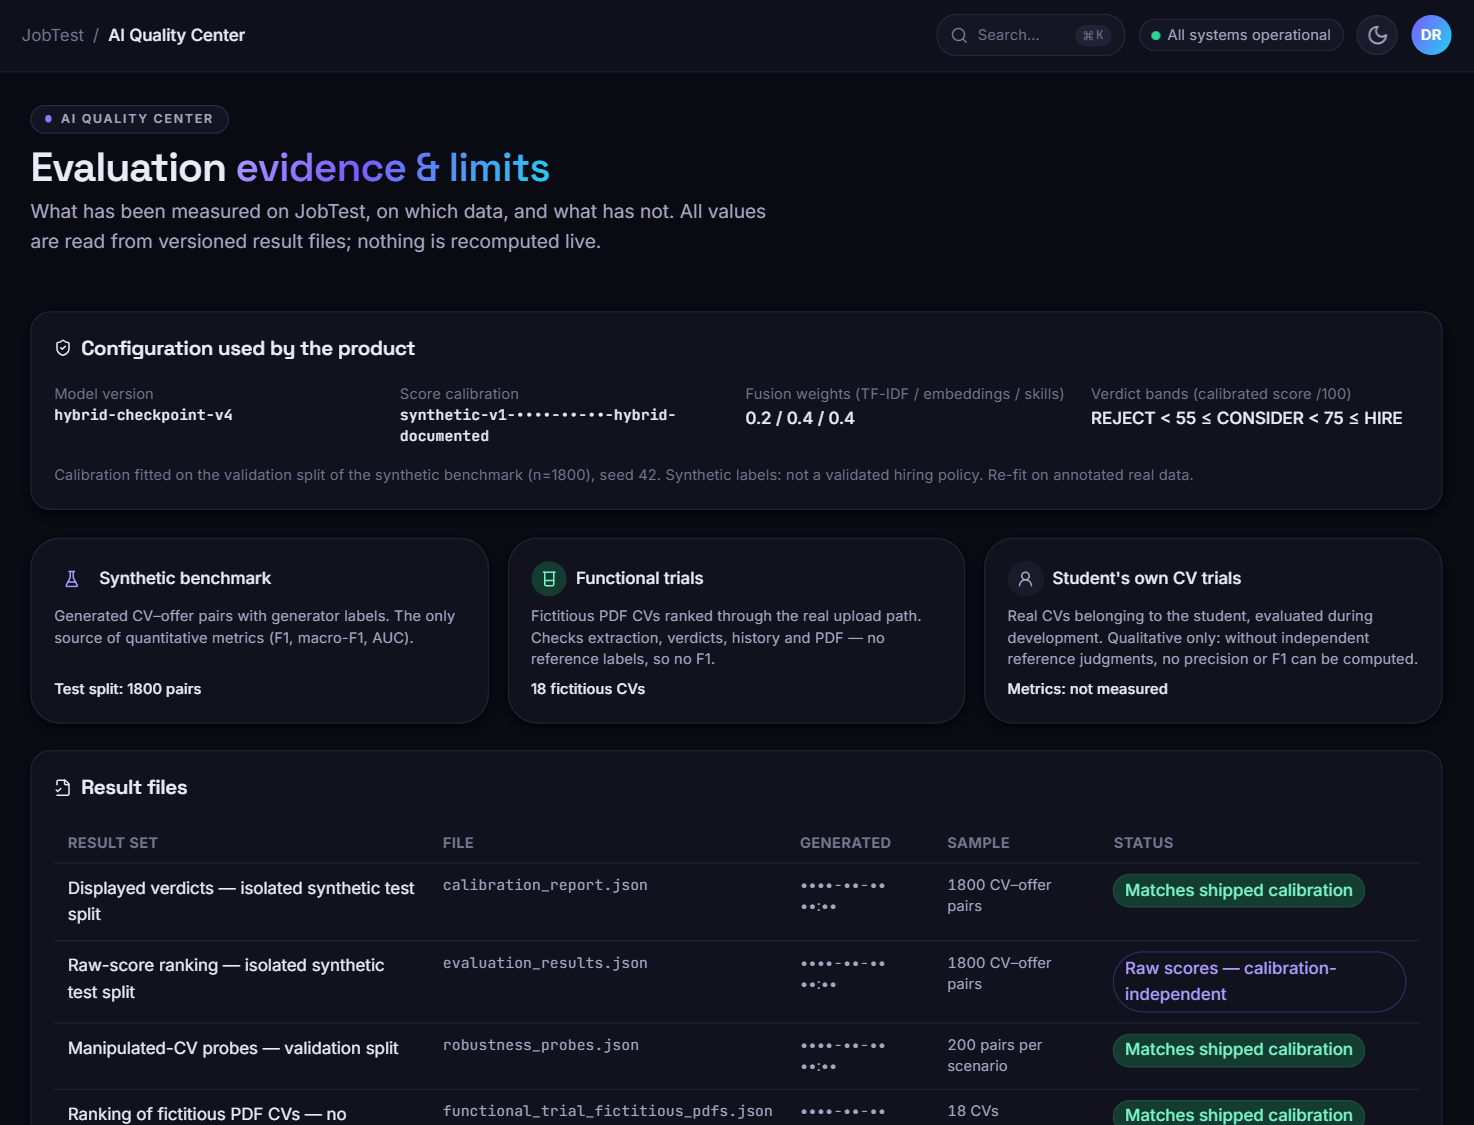
\includegraphics[width=.8\textwidth]{img/interfaces/quality_1.png}
  \caption{\emph{AI Quality Center}~: configuration}
  \label{fig:chap5-quality-1}
\end{figure}

La qualité des verdicts affichés (macro-F1 à trois classes) et la qualité du classement du score brut (F1 binaire à un seuil expérimental) y sont présentées dans deux tableaux distincts, avec leurs définitions et la matrice de confusion de la version livrée (figure~\ref{fig:chap5-quality-2}). Une dernière partie reprend les essais de robustesse face aux CV manipulés (figure~\ref{fig:chap5-quality-3}). Toutes ces valeurs sont lues dans les fichiers versionnés du dossier \texttt{evaluation/results}~; une métrique absente est affichée comme non mesurée, jamais comme nulle.

\begin{figure}[H]
  \centering
  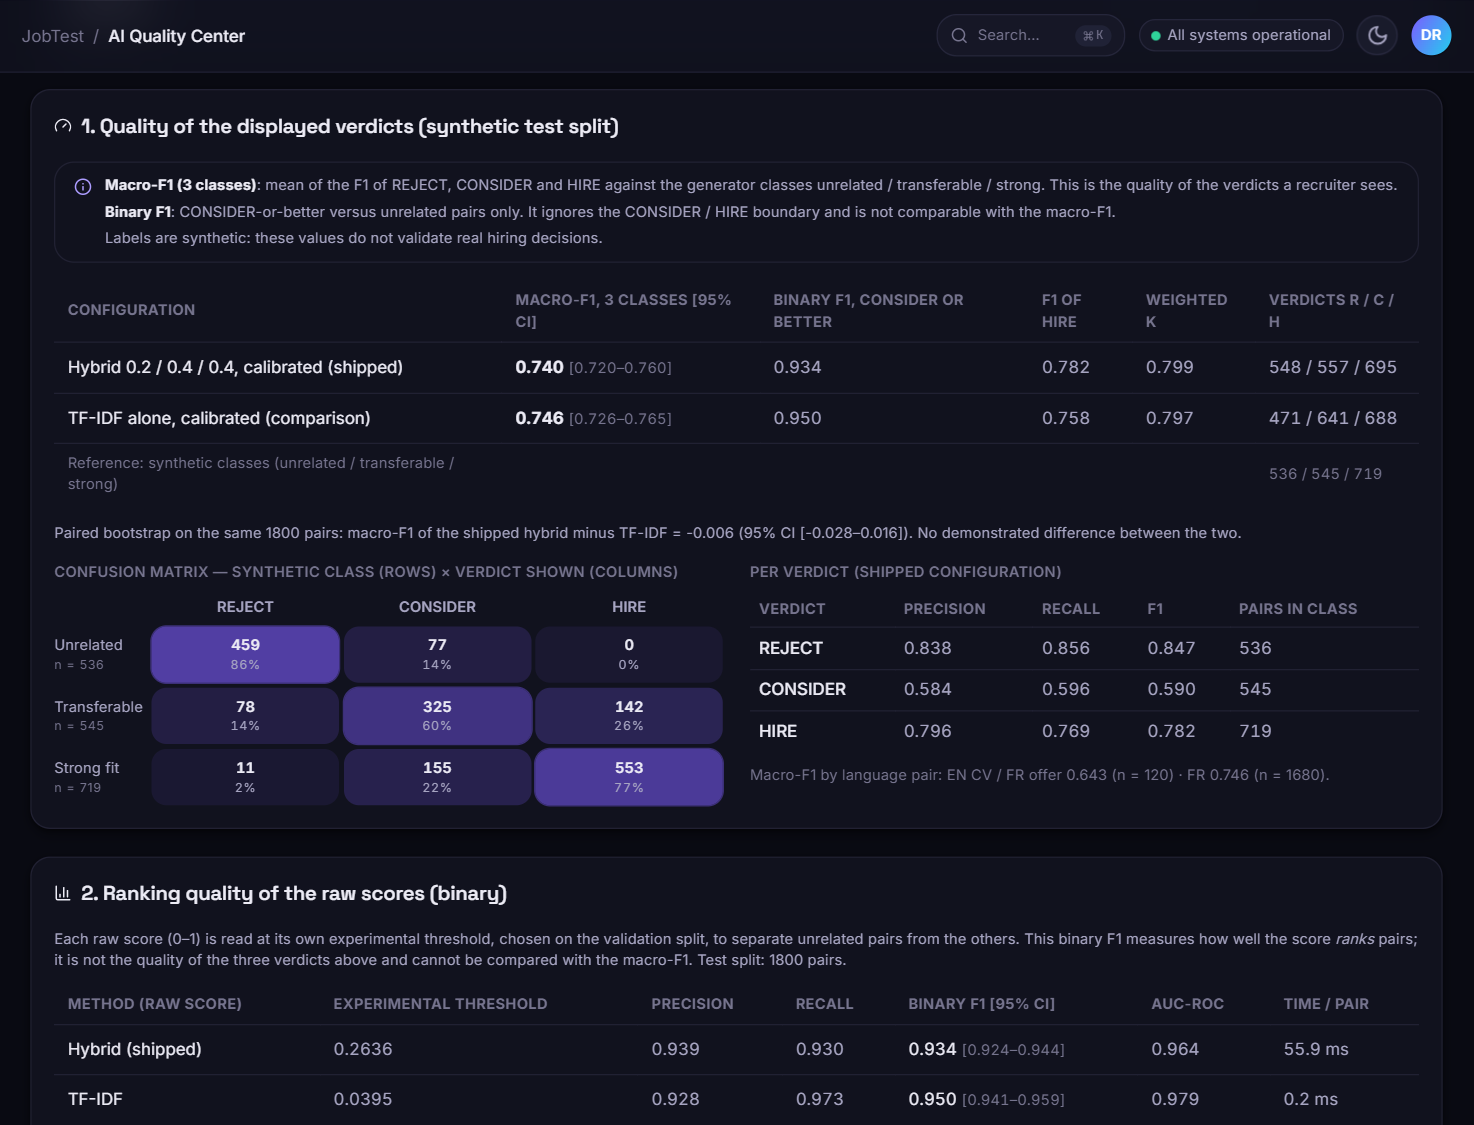
\includegraphics[width=.8\textwidth]{img/interfaces/quality_2.png}
  \caption{\emph{AI Quality Center}~: qualité des verdicts}
  \label{fig:chap5-quality-2}
\end{figure}

\begin{figure}[H]
  \centering
  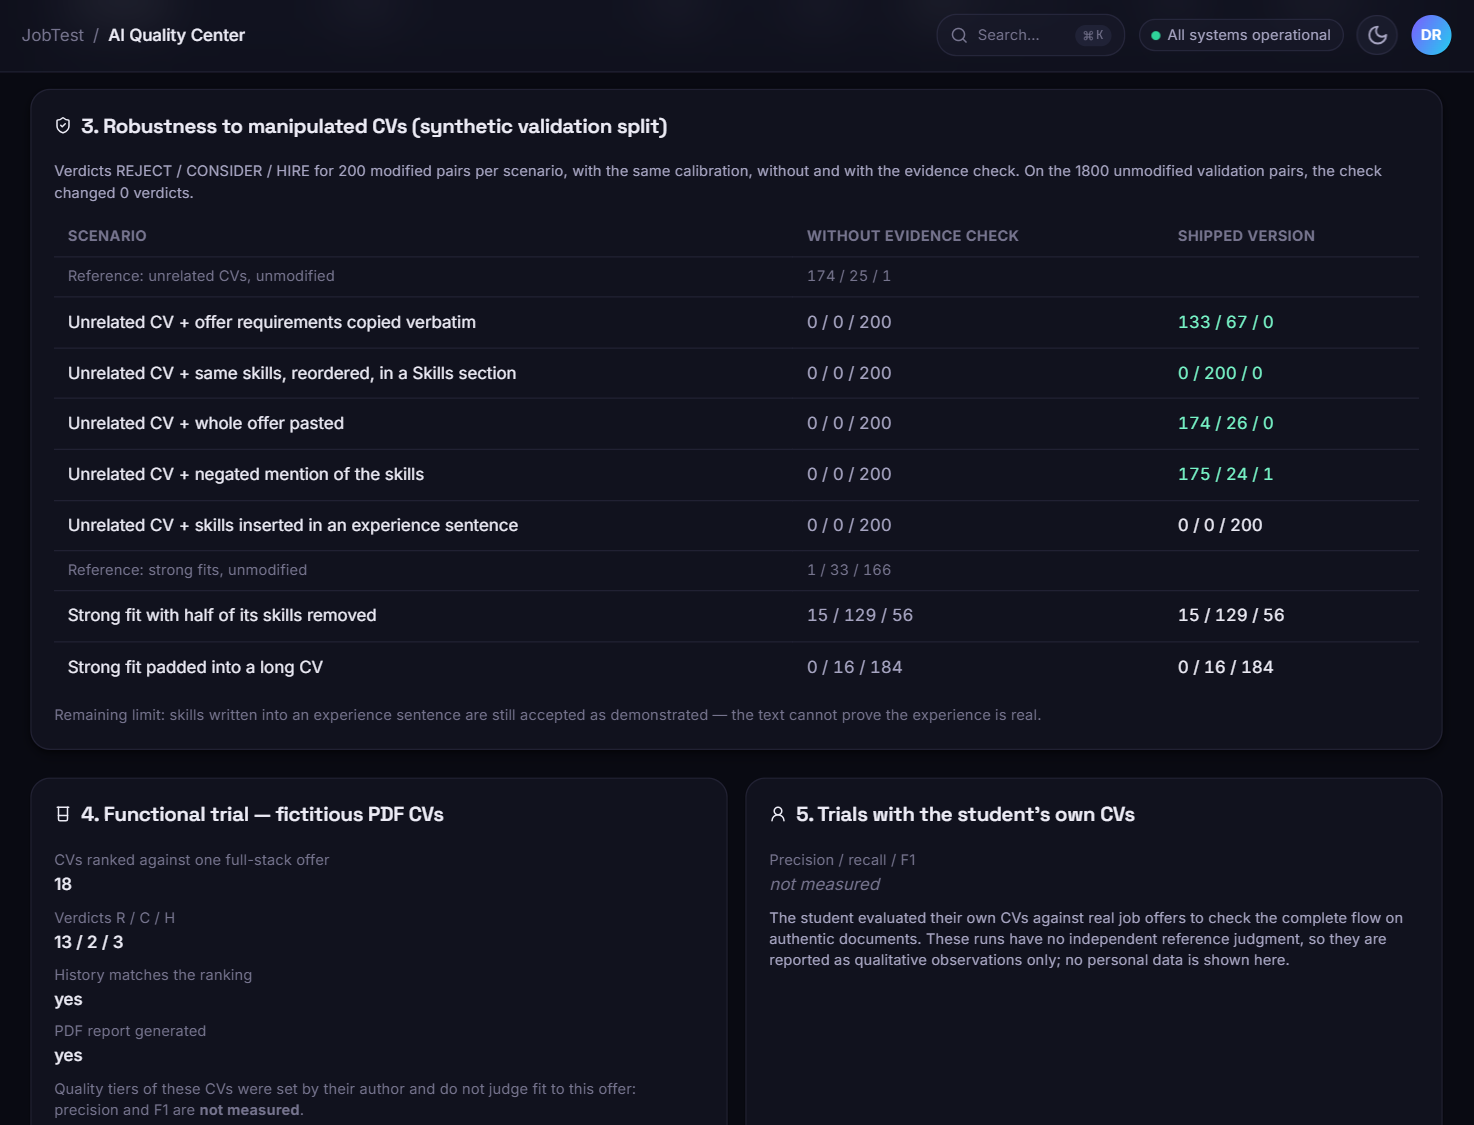
\includegraphics[width=.8\textwidth]{img/interfaces/quality_3.png}
  \caption{\emph{AI Quality Center}~: robustesse}
  \label{fig:chap5-quality-3}
\end{figure}

Enfin, le bouton \emph{Export PDF} de l'écran de résultat déclenche la génération ReportLab et le téléchargement du rapport. Le document reprend les éléments de décision déjà visibles, au lieu de fournir une décision autonome supplémentaire.

\section{Parcours fonctionnel de démonstration}

Un scénario de démonstration se déroule de façon continue : le recruteur se connecte, crée ou sélectionne une offre ouverte, fournit le texte ou le fichier d'un CV, puis lance l'évaluation. Il lit ensuite le score et les raisons associées, consulte si besoin l'analyse approfondie, puis exporte le rapport PDF. L'historique permet enfin de retrouver une évaluation persistée. Ce parcours maintient une séparation claire entre les données métier (offre, candidat et CV), le calcul de correspondance et l'aide à l'interprétation.

\section{Difficultés de réalisation et solutions apportées}

Les difficultés retenues ci-dessous sont celles qui apparaissent dans le code ou dans l'historique technique du projet. Elles concernent la réalisation de la plateforme, non les incidents de déploiement qui seront détaillés au chapitre suivant.

Le tableau~\ref{tab:chap5-difficulties} les présente avec la réponse apportée à chacune.

\begin{table}[H]
\centering
\small
\caption{Difficultés et solutions}
\label{tab:chap5-difficulties}
\begin{tabularx}{\textwidth}{|p{0.27\textwidth}|p{0.28\textwidth}|X|}
\hline
\textbf{Difficulté} & \textbf{Conséquence} & \textbf{Solution retenue}\\
\hline
Prototype Streamlit et interface finale distincts & Risque que le moteur ne soit pas accessible par l'interface Web actuelle. & Création du routeur \texttt{/api/v1/ui}, réutilisant les services métier existants depuis Next.js.\\
\hline
CV PDF et DOCX hétérogènes & Extraction incomplète possible selon le document. & Parsers dédiés avec replis PDF et DOCX avant le prétraitement commun.\\
\hline
Modèles d'embeddings indisponibles ou contraints & Le composant sémantique ne doit pas empêcher le service de répondre. & Chargement différé et stratégie de repli locale documentée dans le moteur.\\
\hline
Layer 2 potentiellement lente ou indisponible & Une réponse LLM ne doit pas bloquer le verdict calculé. & Appel séparé, enveloppe d'état contrôlée et conservation du niveau 1 comme source du score.\\
\hline
Évolution SQLite vers PostgreSQL & Les entités et relations doivent rester cohérentes entre environnements. & Modèles SQLAlchemy communs et configuration par URL de base de données.\\
\hline
Export exploitable hors application & Le recruteur doit partager une synthèse lisible. & Génération serveur ReportLab à partir du résultat déjà obtenu.\\
\hline
\end{tabularx}
\end{table}

\section*{Conclusion}

JobTest est réalisé comme une plateforme Web modulaire dans laquelle Next.js porte le parcours du recruteur et FastAPI centralise les règles métier, les calculs et la persistance. Les écrans transforment un résultat de matching en éléments interprétables : score, compétences, explications, recommandations, analyse qualitative conditionnelle et rapport PDF. Le système soutient ainsi l'évaluation du recruteur sans se substituer à sa décision. Le chapitre suivant présentera les tests, les mesures de sécurité, la conteneurisation et le déploiement Azure.
